% Options for packages loaded elsewhere
\PassOptionsToPackage{unicode}{hyperref}
\PassOptionsToPackage{hyphens}{url}
\PassOptionsToPackage{dvipsnames,svgnames,x11names}{xcolor}
%
\documentclass[
  ignorenonframetext,
]{beamer}
\usepackage{pgfpages}
\setbeamertemplate{caption}[numbered]
\setbeamertemplate{caption label separator}{: }
\setbeamercolor{caption name}{fg=normal text.fg}
\beamertemplatenavigationsymbolsempty
% Prevent slide breaks in the middle of a paragraph
\widowpenalties 1 10000
\raggedbottom
\setbeamertemplate{part page}{
  \centering
  \begin{beamercolorbox}[sep=16pt,center]{part title}
    \usebeamerfont{part title}\insertpart\par
  \end{beamercolorbox}
}
\setbeamertemplate{section page}{
  \centering
  \begin{beamercolorbox}[sep=12pt,center]{part title}
    \usebeamerfont{section title}\insertsection\par
  \end{beamercolorbox}
}
\setbeamertemplate{subsection page}{
  \centering
  \begin{beamercolorbox}[sep=8pt,center]{part title}
    \usebeamerfont{subsection title}\insertsubsection\par
  \end{beamercolorbox}
}
\AtBeginPart{
  \frame{\partpage}
}
\AtBeginSection{
  \ifbibliography
  \else
    \frame{\sectionpage}
  \fi
}
\AtBeginSubsection{
  \frame{\subsectionpage}
}
\usepackage{amsmath,amssymb}
\usepackage{iftex}
\ifPDFTeX
  \usepackage[T1]{fontenc}
  \usepackage[utf8]{inputenc}
  \usepackage{textcomp} % provide euro and other symbols
\else % if luatex or xetex
  \usepackage{unicode-math} % this also loads fontspec
  \defaultfontfeatures{Scale=MatchLowercase}
  \defaultfontfeatures[\rmfamily]{Ligatures=TeX,Scale=1}
\fi
\usepackage{lmodern}
\ifPDFTeX\else
  % xetex/luatex font selection
\fi
% Use upquote if available, for straight quotes in verbatim environments
\IfFileExists{upquote.sty}{\usepackage{upquote}}{}
\IfFileExists{microtype.sty}{% use microtype if available
  \usepackage[]{microtype}
  \UseMicrotypeSet[protrusion]{basicmath} % disable protrusion for tt fonts
}{}
\makeatletter
\@ifundefined{KOMAClassName}{% if non-KOMA class
  \IfFileExists{parskip.sty}{%
    \usepackage{parskip}
  }{% else
    \setlength{\parindent}{0pt}
    \setlength{\parskip}{6pt plus 2pt minus 1pt}}
}{% if KOMA class
  \KOMAoptions{parskip=half}}
\makeatother
\usepackage{xcolor}
\newif\ifbibliography
\setlength{\emergencystretch}{3em} % prevent overfull lines
\providecommand{\tightlist}{%
  \setlength{\itemsep}{0pt}\setlength{\parskip}{0pt}}
\setcounter{secnumdepth}{-\maxdimen} % remove section numbering
\newlength{\cslhangindent}
\setlength{\cslhangindent}{1.5em}
\newlength{\csllabelwidth}
\setlength{\csllabelwidth}{3em}
\newlength{\cslentryspacingunit} % times entry-spacing
\setlength{\cslentryspacingunit}{\parskip}
\newenvironment{CSLReferences}[2] % #1 hanging-ident, #2 entry spacing
 {% don't indent paragraphs
  \setlength{\parindent}{0pt}
  % turn on hanging indent if param 1 is 1
  \ifodd #1
  \let\oldpar\par
  \def\par{\hangindent=\cslhangindent\oldpar}
  \fi
  % set entry spacing
  \setlength{\parskip}{#2\cslentryspacingunit}
 }%
 {}
\usepackage{calc}
\newcommand{\CSLBlock}[1]{#1\hfill\break}
\newcommand{\CSLLeftMargin}[1]{\parbox[t]{\csllabelwidth}{#1}}
\newcommand{\CSLRightInline}[1]{\parbox[t]{\linewidth - \csllabelwidth}{#1}\break}
\newcommand{\CSLIndent}[1]{\hspace{\cslhangindent}#1}
\ifLuaTeX
\usepackage[bidi=basic]{babel}
\else
\usepackage[bidi=default]{babel}
\fi
\babelprovide[main,import]{spanish}
% get rid of language-specific shorthands (see #6817):
\let\LanguageShortHands\languageshorthands
\def\languageshorthands#1{}
\ifLuaTeX
  \usepackage{selnolig}  % disable illegal ligatures
\fi
\IfFileExists{bookmark.sty}{\usepackage{bookmark}}{\usepackage{hyperref}}
\IfFileExists{xurl.sty}{\usepackage{xurl}}{} % add URL line breaks if available
\urlstyle{same}
\hypersetup{
  pdftitle={Egresos del Sector Público},
  pdfauthor={Ignacio Campón},
  pdflang={es},
  colorlinks=true,
  linkcolor={blue},
  filecolor={Maroon},
  citecolor={blue},
  urlcolor={blue},
  pdfcreator={LaTeX via pandoc}}

\title{Egresos del Sector Público}
\subtitle{Series Cronológicas}
\author{Ignacio Campón}
\date{2024-07-05}

\begin{document}
\frame{\titlepage}

\begin{frame}{Introduccion}
\protect\hypertarget{introduccion}{}
Los \textbf{Egresos Primarios del Sector Público no Monetario}, son una
fuente crucial de información proporcionada por el
\href{https://www.gub.uy/ministerio-economia-finanzas/datos-y-estadisticas/estadisticas/informacion-resultados-del-sector-publico}{Ministerio
de Economía y Finanzas}. Esta serie mensual, ofrece una panorámica
detallada de los desembolsos financieros del sector público, a lo largo
del tiempo.

Los egresos primarios del sector público son fundamentales para entender
la dinámica fiscal de un país, ya que representan los gastos esenciales
en bienes y servicios no financieros realizados por el gobierno. Estos
datos son vitales para analizar la gestión presupuestaria, evaluar
políticas económicas y anticipar tendencias futuras en base a modelos
estadísticos.

Se explorará la serie temporal con el objetivo de identificar un modelo
adecuado que permita reproducirl, facilitando así la capacidad
predictiva sobre los egresos del sector público en Uruguay.
\end{frame}

\begin{frame}{Serie temporal: Gasto Público}
\protect\hypertarget{serie-temporal-gasto-puxfablico}{}
\begin{figure}[H]

{\centering 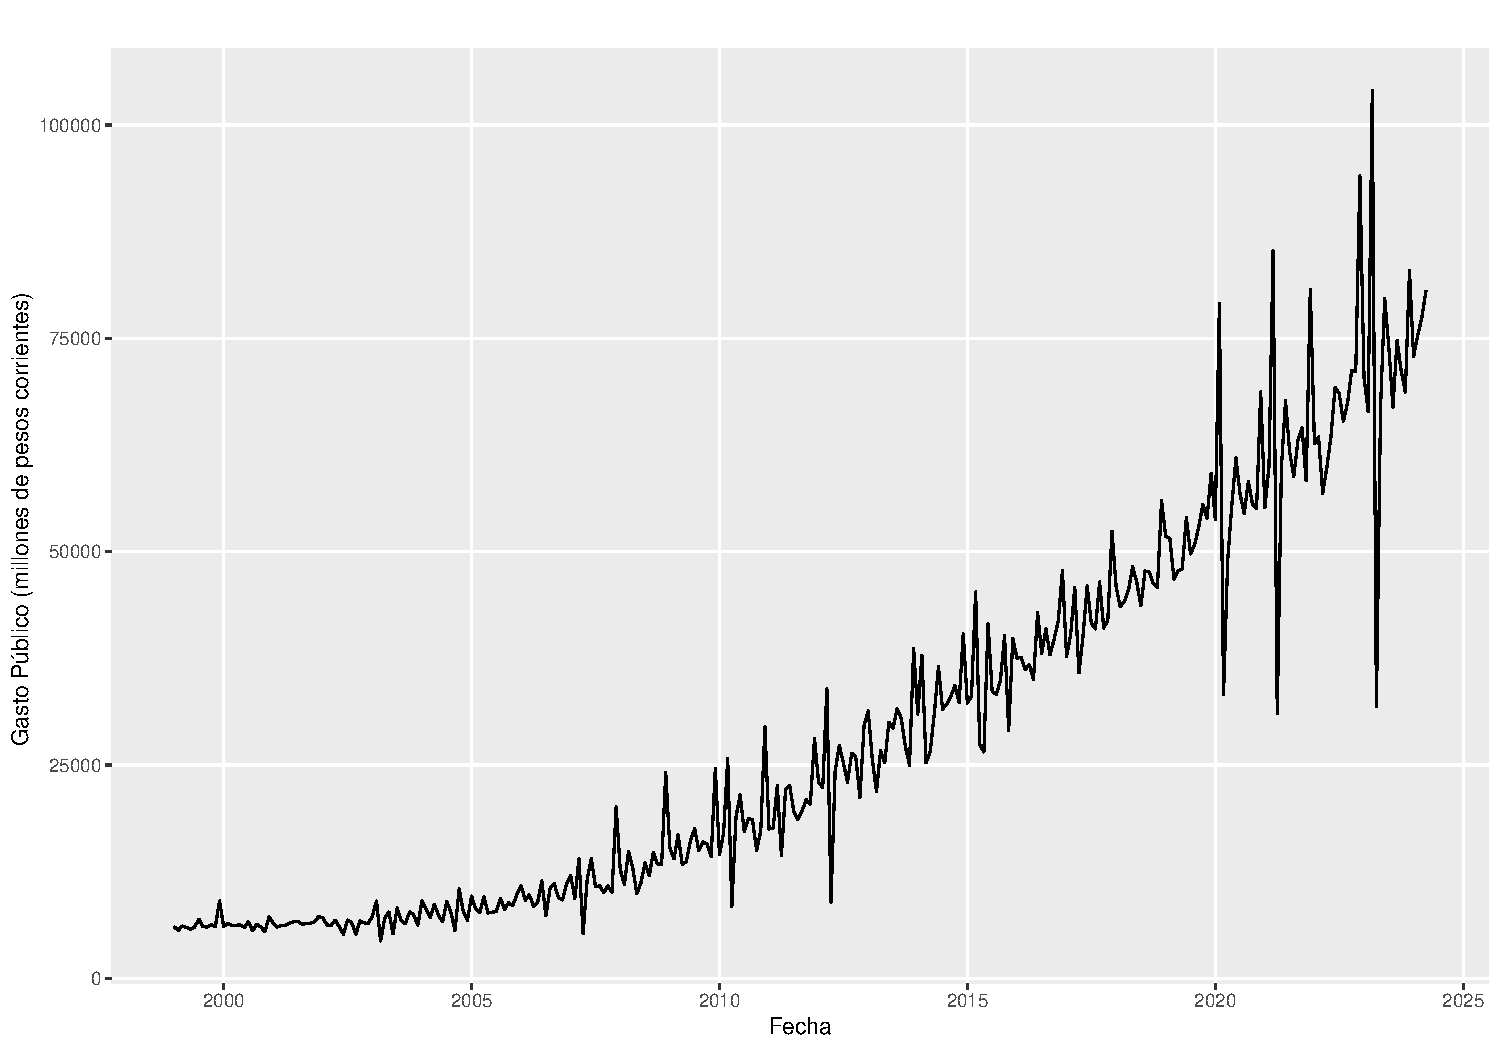
\includegraphics[width=0.85\linewidth]{presentacion_files/figure-beamer/plot_series_inicial-1} 

}

\caption{\label{gasto_publico} Evolución del Gasto Público mensual en millones de pesos corrientes entre enero 1999 y abril 2024.}\label{fig:plot_series_inicial}
\end{figure}
\end{frame}

\begin{frame}{Análisis descriptivo}
\protect\hypertarget{anuxe1lisis-descriptivo}{}
\begin{figure}[H]

{\centering 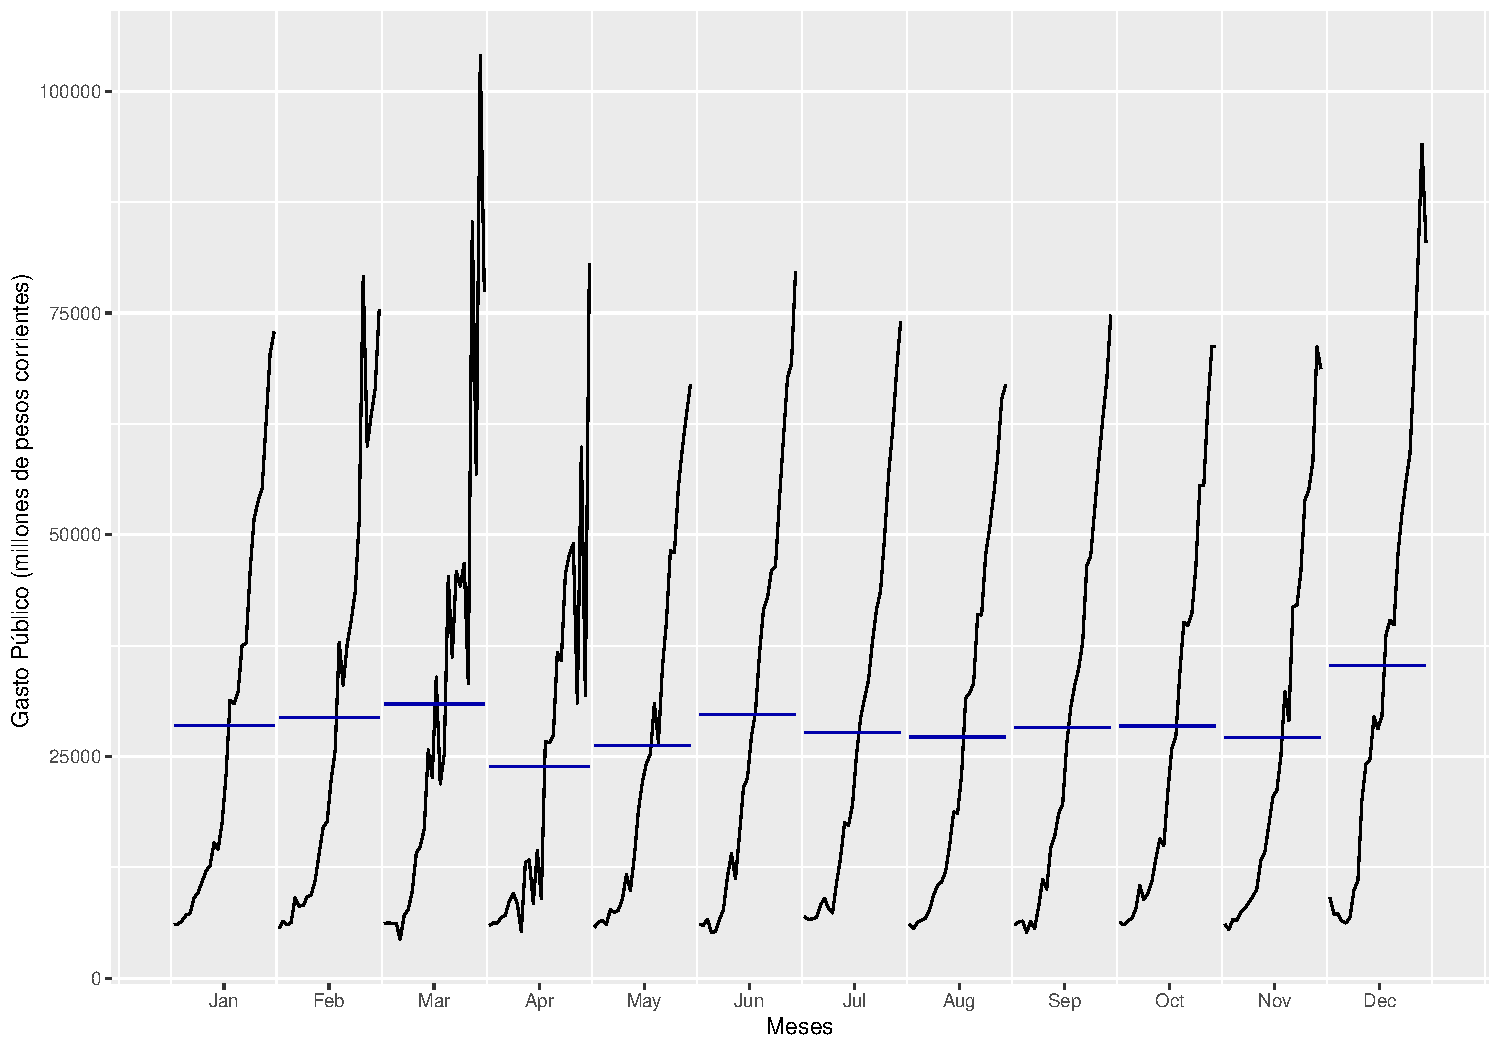
\includegraphics[width=0.85\linewidth]{presentacion_files/figure-beamer/month_plot-1} 

}

\caption{\label{month_plot} Comportamiento mensual del Gasto Público entre 1999 y 2024.}\label{fig:month_plot}
\end{figure}
\end{frame}

\begin{frame}{Análisis descriptivo (2)}
\protect\hypertarget{anuxe1lisis-descriptivo-2}{}
\begin{figure}[H]

{\centering 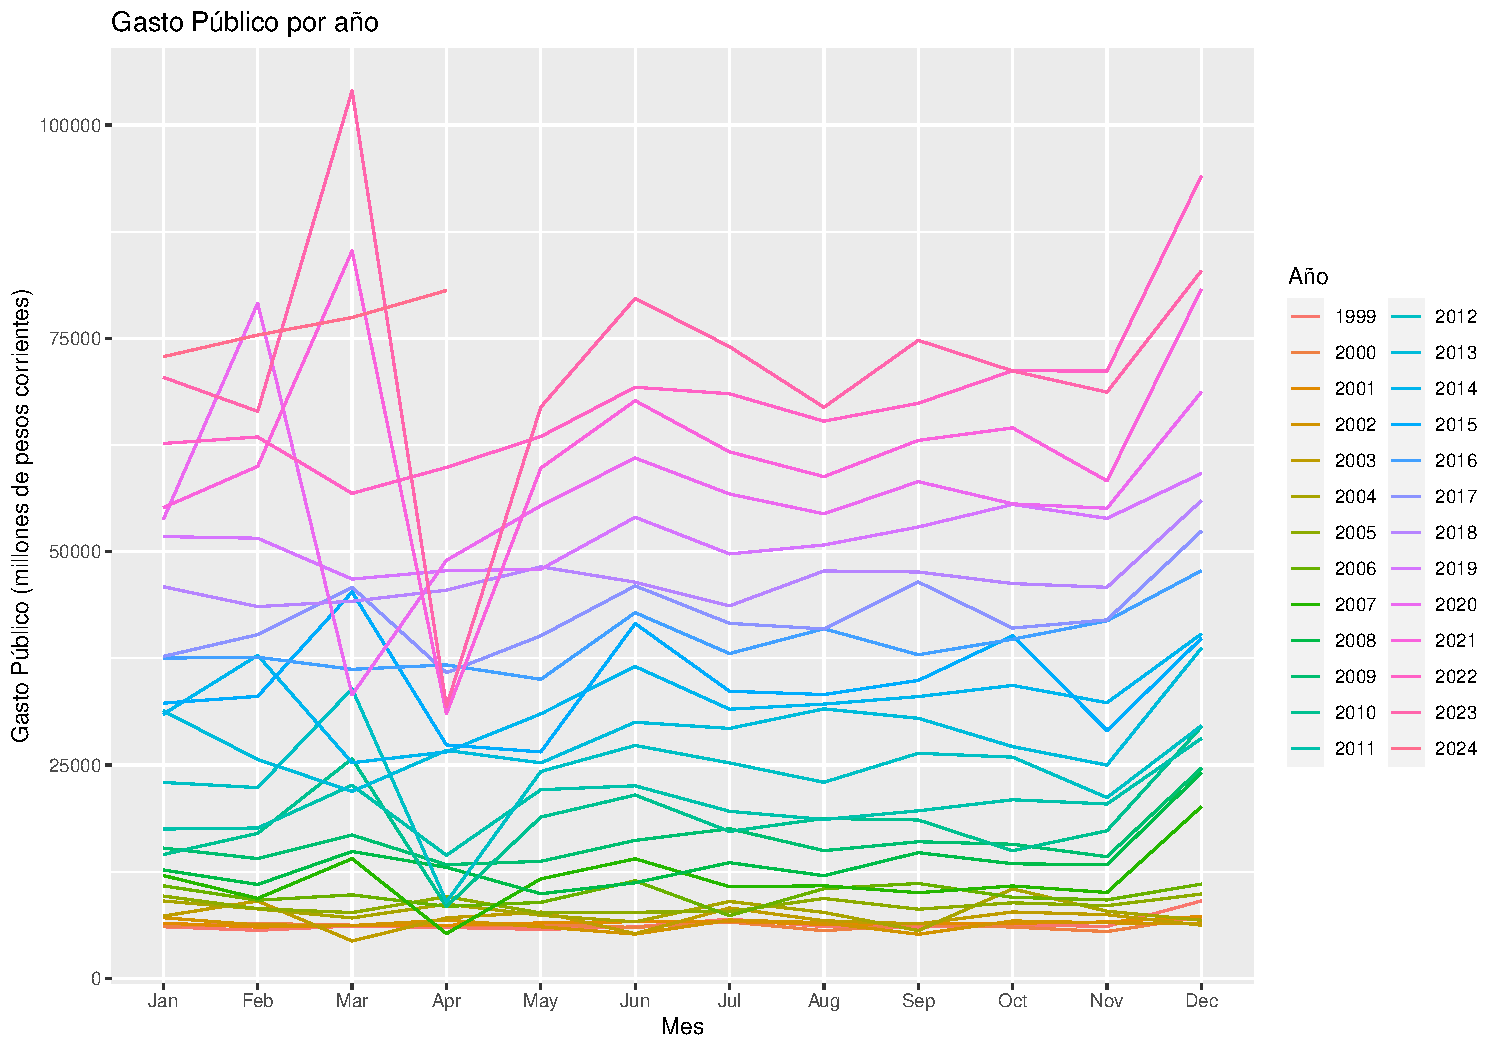
\includegraphics[width=0.85\linewidth]{presentacion_files/figure-beamer/season_plot-1} 

}

\caption{\label{seasonal_plot} Comportamiento por año del Gasto Público entre 1999 y 2024.}\label{fig:season_plot}
\end{figure}
\end{frame}

\begin{frame}{Metodología}
\protect\hypertarget{metodologia}{}
El desarrollo esta basado en la metodología de Box y Jenkins, en la
construcción de modelos ARIMA para el análisis de series de tiempo.
Podemos dividir esta metodología en cuatro grandes etapas:

\begin{itemize}
\item
  identificación
\item
  estimación
\item
  diagnostico
\item
  predicción
\end{itemize}
\end{frame}

\begin{frame}{Metodología (2)}
\protect\hypertarget{metodologuxeda-2}{}
La identificación del modelo, esta basada en las funciones de
autocorrelación y autocorrelación parcial y a partir de ello, podremos
obtener diferentes modelos candidatos. Tras la estimación, un
diagnostico con determinadas etapas es realizado; y por último,
aplicaremos predicciones sobre los mismos y se evaluará su desempeño.
\end{frame}

\begin{frame}{Logaritmo de la serie}
\protect\hypertarget{logaritmo-de-la-serie}{}
\begin{figure}[H]

{\centering 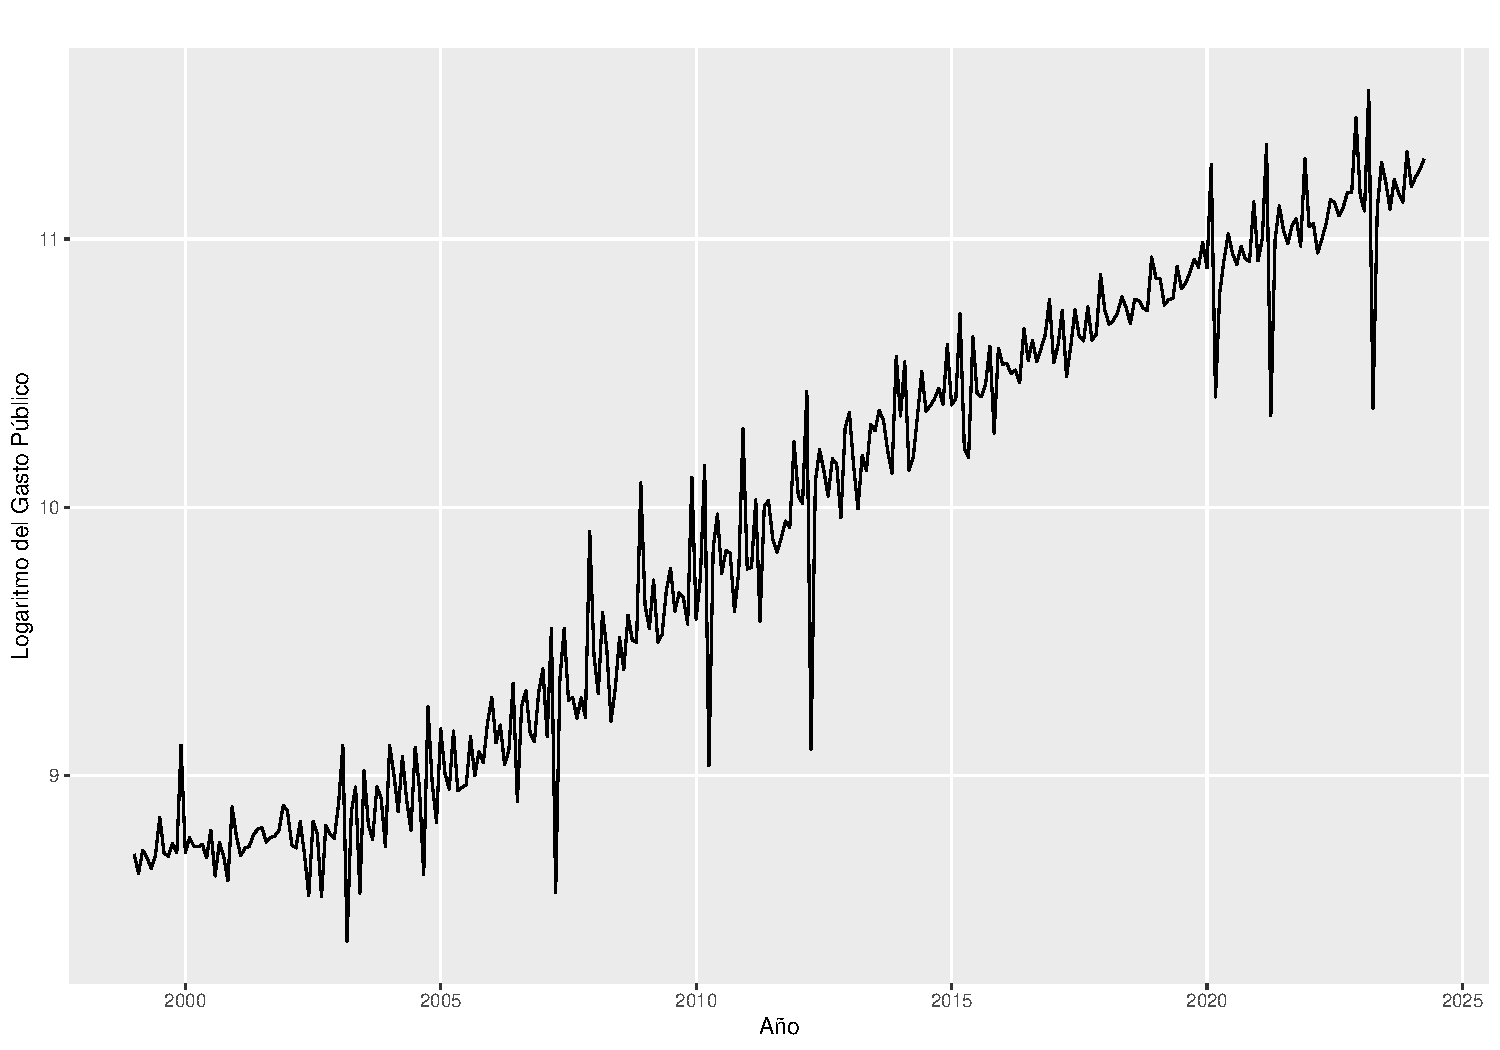
\includegraphics[width=0.85\linewidth]{presentacion_files/figure-beamer/log_plot-1} 

}

\caption{\label{log_plot} Evolución del logaritmo del Gasto Público mensual entre 1999 y 2024.}\label{fig:log_plot}
\end{figure}
\end{frame}

\begin{frame}{Funciones de Autocorrelación}
\protect\hypertarget{funciones-de-autocorrelaciuxf3n}{}
\begin{figure}[H]

{\centering 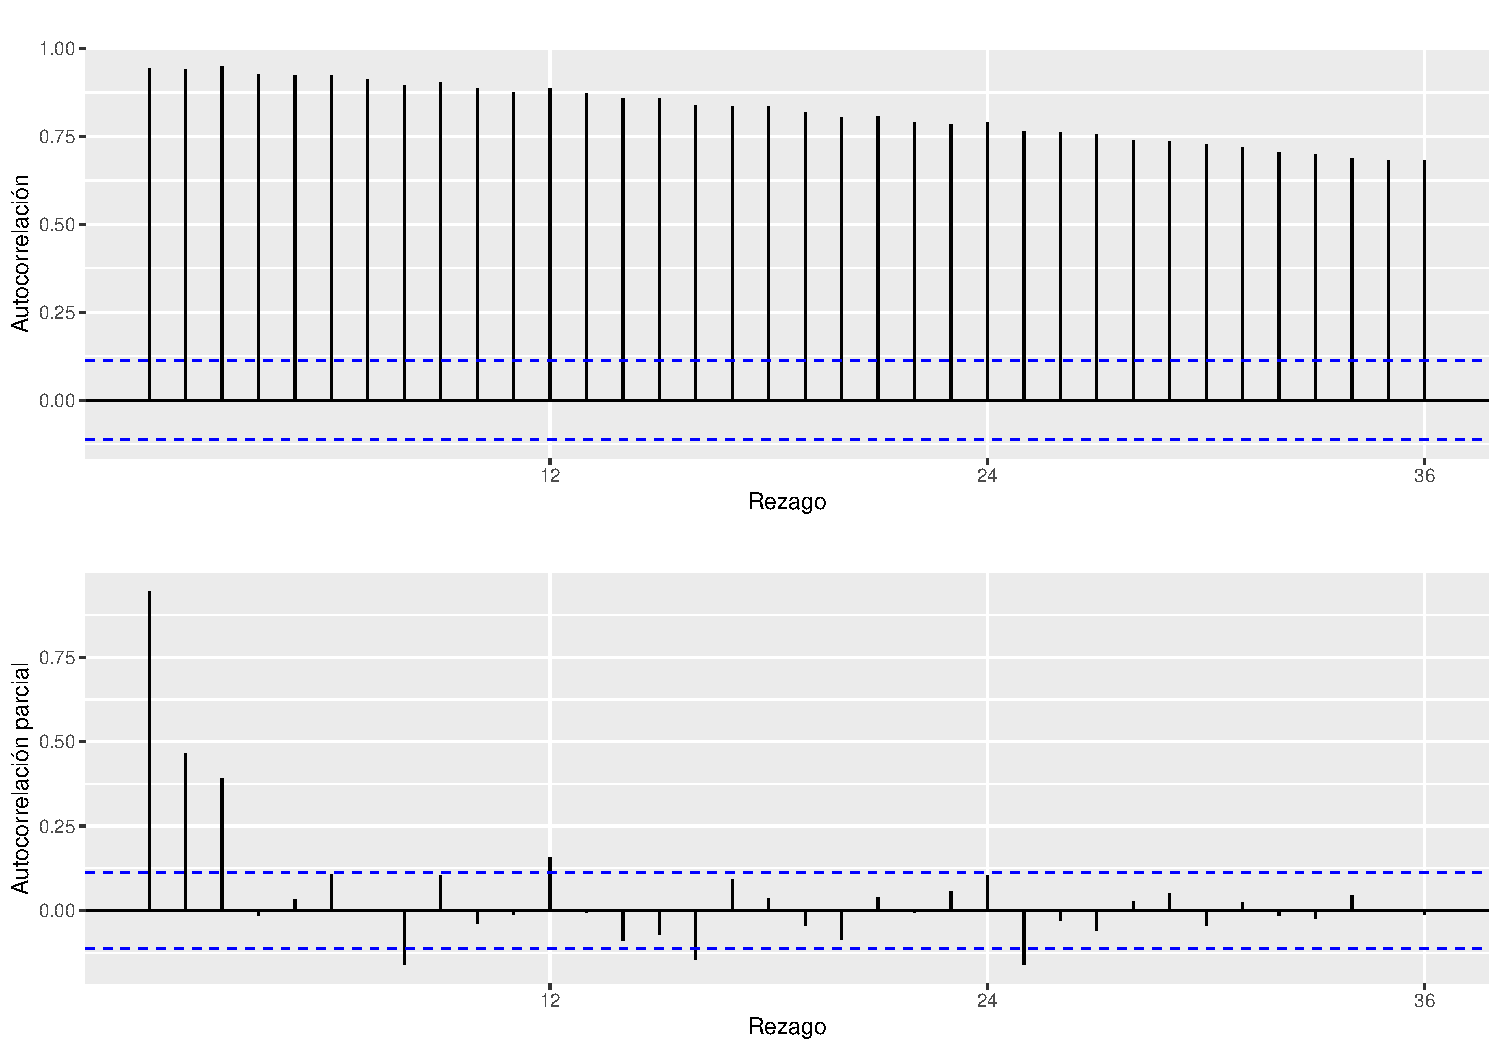
\includegraphics[width=0.85\linewidth]{presentacion_files/figure-beamer/unnamed-chunk-1-1} 

}

\caption{\label{fac_facp} Funciones de Autocorrelación y Autocorrelación Parcial estimadas del logaritmo del Gasto Público.}\label{fig:unnamed-chunk-1}
\end{figure}
\end{frame}

\begin{frame}{Test de Dickey-Fuller}
\protect\hypertarget{test-de-dickey-fuller}{}
Este test contrasta en su hipótesis nula que el proceso contiene una
raíz unitaria y por lo tanto que es no estacionario, mientras que la
alternativa es que no presenta raíz unitaria y por lo tanto, se cumple
el supuesto de estacionariedad.

La siguiente ecuación es la regresión auxiliar con tendencia
determínistica para la solución paramétrica de DF (1979):

\[ \Delta Y_t = a_0 + a_2 t + \gamma Y_{t-1} + \sum_{j=1}^{k} \beta_j \Delta Y_{t-j} + \epsilon_t \]
donde \(Y_t\) es la serie de tiempo, \(t\) es el tiempo, \(\Delta\) es
el operador de diferencia, \(a_0\) y \(a_2\) son los coeficientes de la
regresión, \(\gamma\) es el coeficiente de la raíz unitaria, \(\beta_j\)
son los coeficientes de los rezagos y \(\epsilon_t\) es el término de
error.
\end{frame}

\begin{frame}{Test de Dickey-Fuller (2)}
\protect\hypertarget{test-de-dickey-fuller-2}{}
Los contrastes de hipótesis que se realizan son los siguientes tres:

\begin{itemize}
\tightlist
\item
  Estadístico de prueba, \(\tau_3\) contrasta la hipótesis nula de que
  hay raíz unitaria, contra la alternativa de que no hay raíz unitaria,
  es decir es un proceso estacionario.
\end{itemize}

\begin{align*}
& \mathbf{H_0} : \gamma = 0 \\
& \mathbf{H_1} : \gamma < 1
\end{align*}

\begin{itemize}
\tightlist
\item
  Estadístico de prueba, \(\phi_2\) contrasta la hipótesis nula de que
  no tiene raíz unitaria, constante ni tendencia, contra la alternativa
  de que una de ellas es distinta de 0.
\end{itemize}

\begin{align*}
& \mathbf{H_0} : \gamma = a_0 = a_2 = 0 \\
& \mathbf{H_1} : \text{Al menos uno de ellos es distinto de 0.}
\end{align*}
\end{frame}

\begin{frame}{Test de Dickey-Fuller (3)}
\protect\hypertarget{test-de-dickey-fuller-3}{}
\begin{itemize}
\tightlist
\item
  Estadístico de prueba, \(\phi_3\) contrasta la hipótesis nula de que
  no tiene raíz unitaria ni tendencia, contra la alternativa de que una
  de ellas es distinta de 0.
\end{itemize}

\begin{align*}
& \mathbf{H_0} : \gamma = a_2 = 0 \\
& \mathbf{H_1} : \text{Al menos uno de ellos es distinto de 0.}
\end{align*}

El estadístico \(\tau_3\) bajo la hipótesis nula sigue una distribución
t-Student, mientras que los estadísticos \(\phi_2\) y \(\phi_3\) de
prueba conjunta siguen una distribución F de Fisher.
\end{frame}

\begin{frame}{Test de Dickey-Fuller (4)}
\protect\hypertarget{test-de-dickey-fuller-4}{}
Se aplica el test de Dickey-Fuller sobre el logarítmo del gasto público.
El test con tendencia y 12 rézagos significativos obtuvo los siguientes
resultados para un nivel de significación al 5\%. El estadístico
\(\tau_3 = -2.33\) y un \(p-valor=-3.42\), no se rechaza \(H_0\) y por
lo tanto la serie tiene una raíz unitaria. Luego, \(\phi_2 = 20.29\) y
un \(p-valor=4.71\), se rechaza \(H_0\), por lo tanto al menos uno de
\(\gamma = a_0 = a_2\) es distinto de 0, es decir o presenta constante,
o presenta tendencia, porque ya se constrasto que \(\gamma = 0\). Por
último, \(\phi_3 = 3.13\) y un \(p-valor=6.30\), no se rechaza \(H_0\),
entonces \(\gamma\) o \(a_0\) es distinto de 0.

Por lo tanto, dado los 3 contrastes se concluye que la serie tiene raíz
unitaria, no tiene tendencia y presenta constante. Esto sugiere que la
serie no es estacionaria y se debe de aplicar una diferencia regular
para obtener un proceso estacionario.
\end{frame}

\begin{frame}{Diferencia regular}
\protect\hypertarget{diferencia-regular}{}
\[(1-L)Ln(gasto)\]

\begin{figure}[H]

{\centering 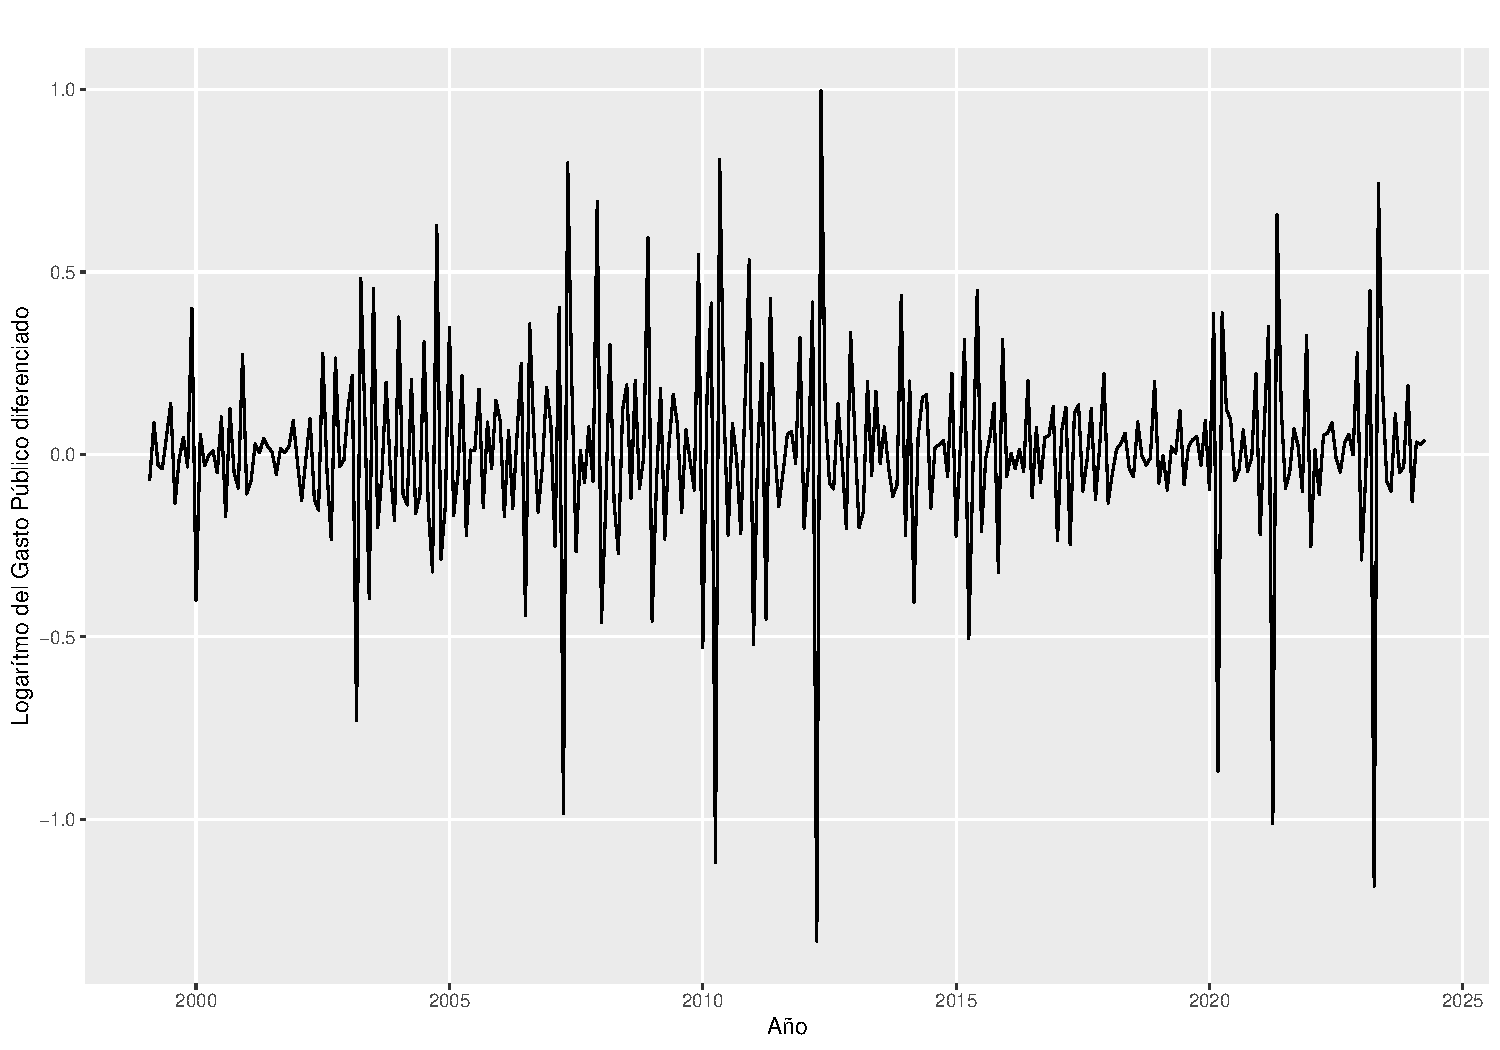
\includegraphics[width=0.75\linewidth]{presentacion_files/figure-beamer/unnamed-chunk-2-1} 

}

\caption{\label{diff_plot} Evolución de la primera diferencia regular del logaritmo del Gasto Público mensual entre 1999 y 2024.}\label{fig:unnamed-chunk-2}
\end{figure}
\end{frame}

\begin{frame}{Funciones de Autocorrelación serie diferenciada}
\protect\hypertarget{funciones-de-autocorrelaciuxf3n-serie-diferenciada}{}
\begin{figure}[H]

{\centering 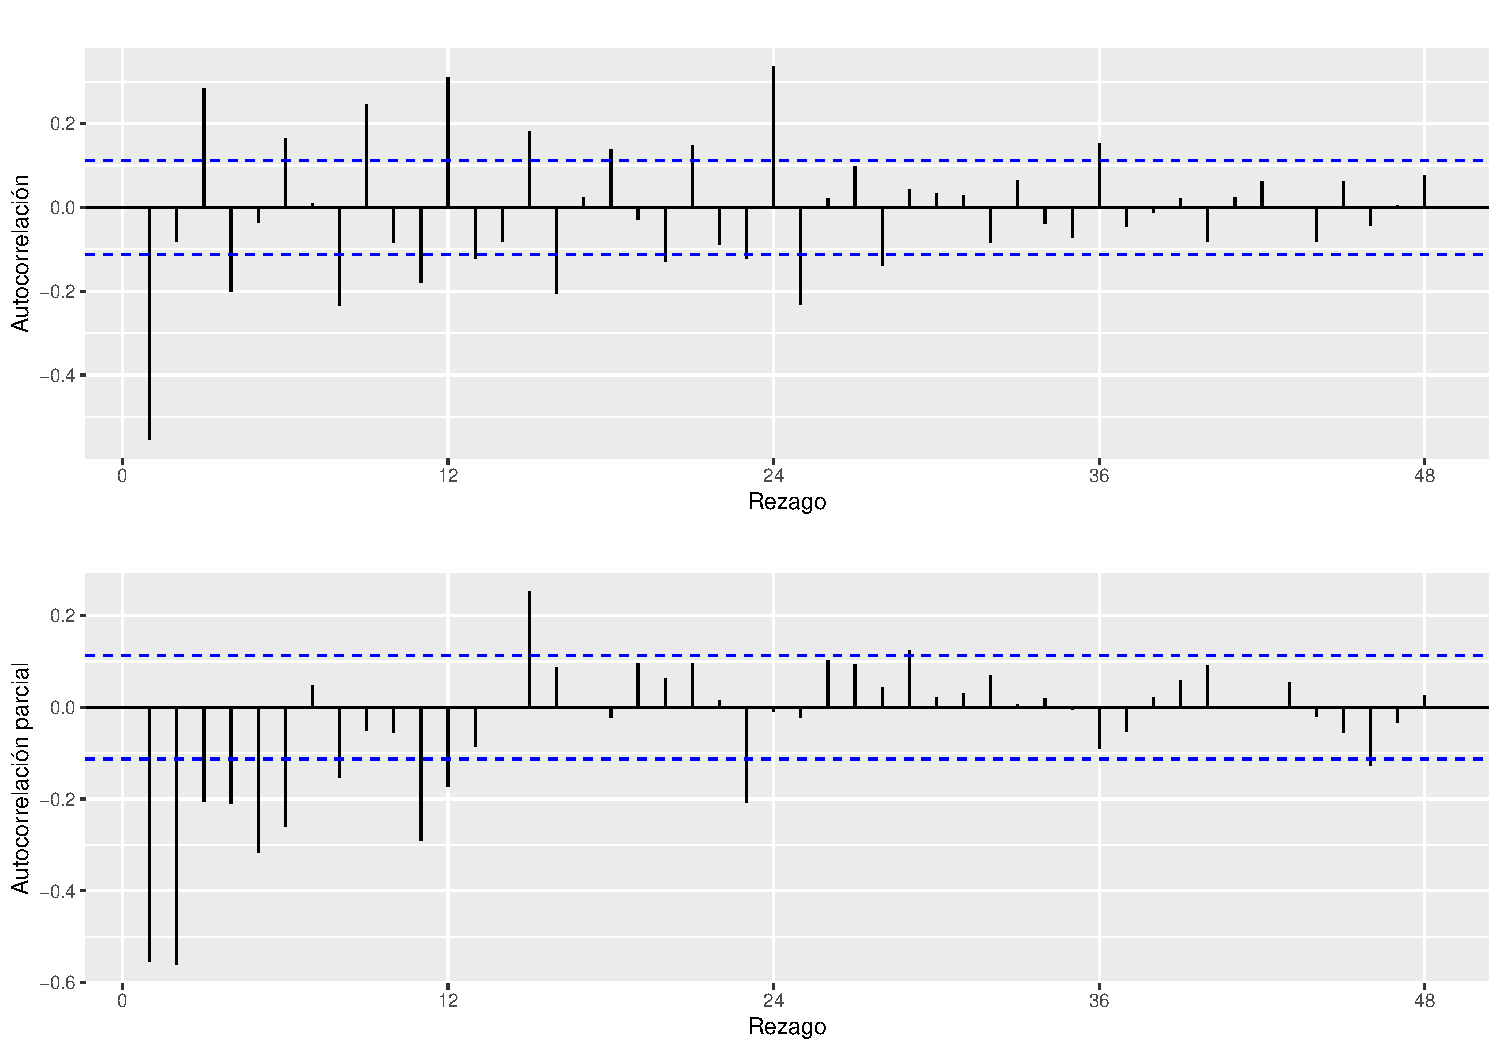
\includegraphics[width=0.85\linewidth]{presentacion_files/figure-beamer/unnamed-chunk-3-1} 

}

\caption{\label{fac_facp_diff} Funciones de Autocorrelación y Autocorrelación Parcial estimadas para la primera diferencia regular del logaritmo del Gasto Público.}\label{fig:unnamed-chunk-3}
\end{figure}
\end{frame}

\begin{frame}{Diferencia estacional}
\protect\hypertarget{diferencia-estacional}{}
\[(1-L^{12}) Ln(gasto)\]

\begin{figure}[H]

{\centering 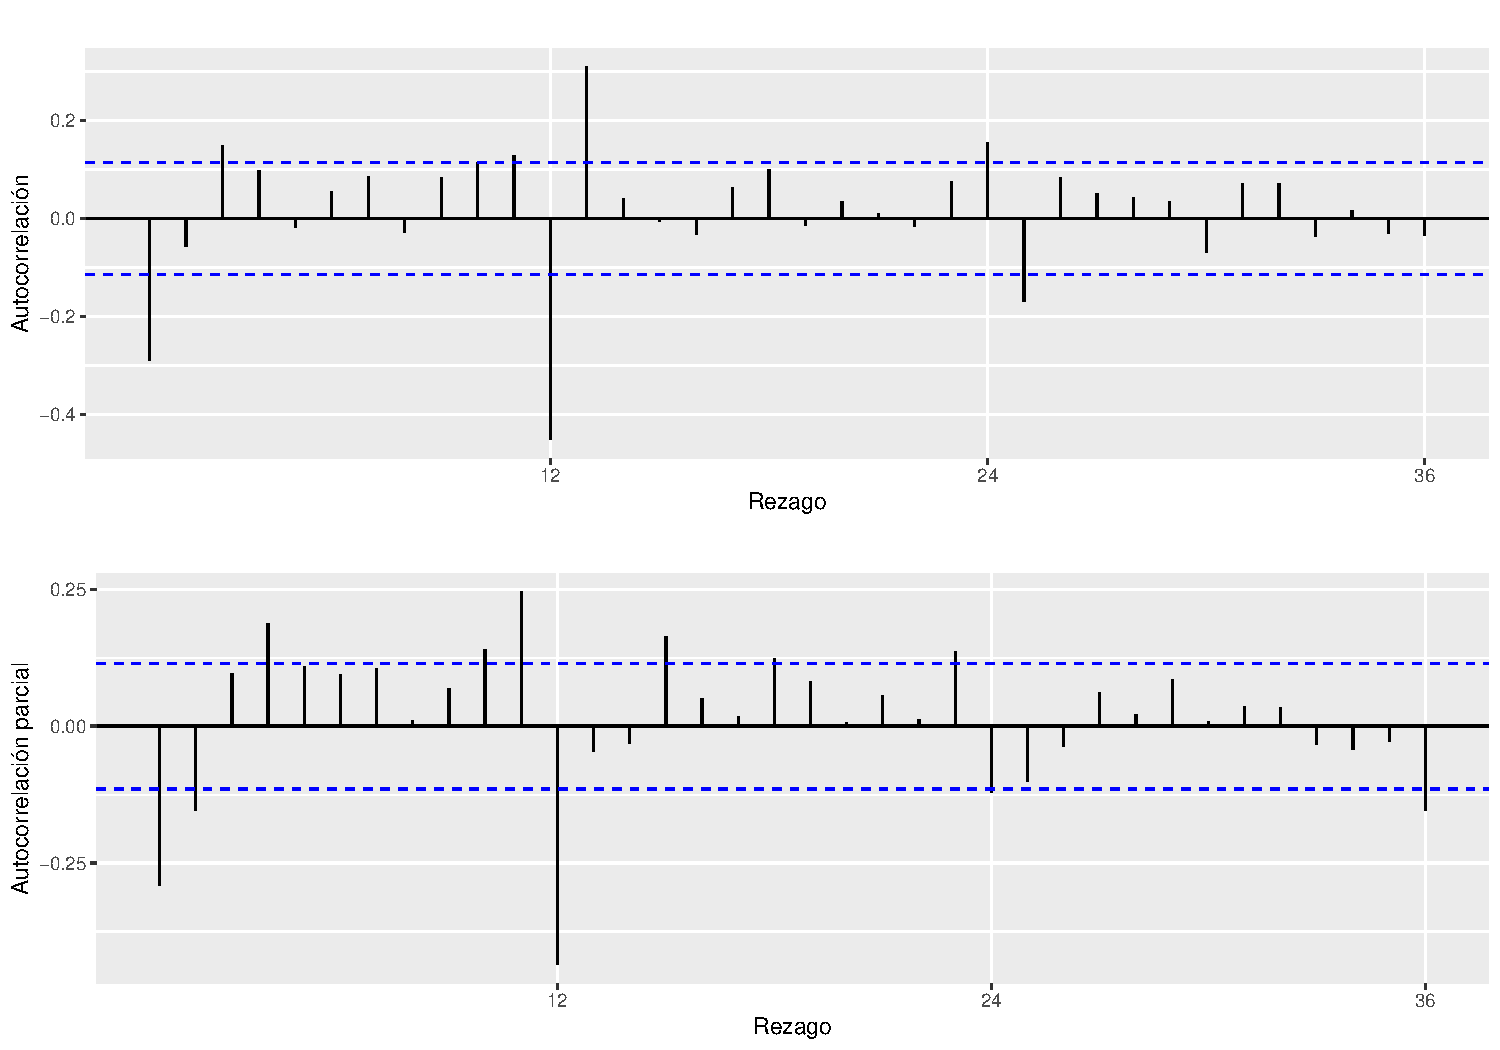
\includegraphics[width=0.7\linewidth]{presentacion_files/figure-beamer/unnamed-chunk-4-1} 

}

\caption{\label{fac_facp_estac} Funciones de Autocorrelación y Autocorrelación Parcial estimadas para la primera diferencia estacional del logaritmo del Gasto Público (1999-2024).}\label{fig:unnamed-chunk-4}
\end{figure}
\end{frame}

\begin{frame}{Identificación}
\protect\hypertarget{identificaciuxf3n}{}
Se identifican dos modelos posibles, \textbf{SARIMA(0,0,1)(0,1,1)} y
\textbf{SARIMA(0,0,1)(1,1,0)}.

Estos modelos surgen de los rezagos significativos presentes en las
funciones. Con respecto a la parte regular de modelo, se puede observar
una rápida convergencia de la serie en la FAC, mientras que en la FACP
dicha convergencia no es tan rápida, lo cual sugiere un modelo que
contiene solo parte MA; el rezago 1 significativo de la FAC sugiere
\(q=1\) y \(p=d=0\) en un modelo SARIMA(p,d,q)(P,D,Q). Con respecto a la
parte estacional, los rezagos múltiplos de 12 son los relevantes en la
FAC y FACP, ambas funciones presentan el primer rezago (rezago 12)
significativo, y una convergencia medianamente rápida. Esto sugiere
probar dos posibilidades \(P=1\) o \(Q=1\) siendo \(D=1\).
\end{frame}

\begin{frame}{Diferencia regular y estacional}
\protect\hypertarget{diferencia-regular-y-estacional}{}
\[(1-L)(1-L^{12}) Ln(gasto)\]

\begin{figure}[H]

{\centering 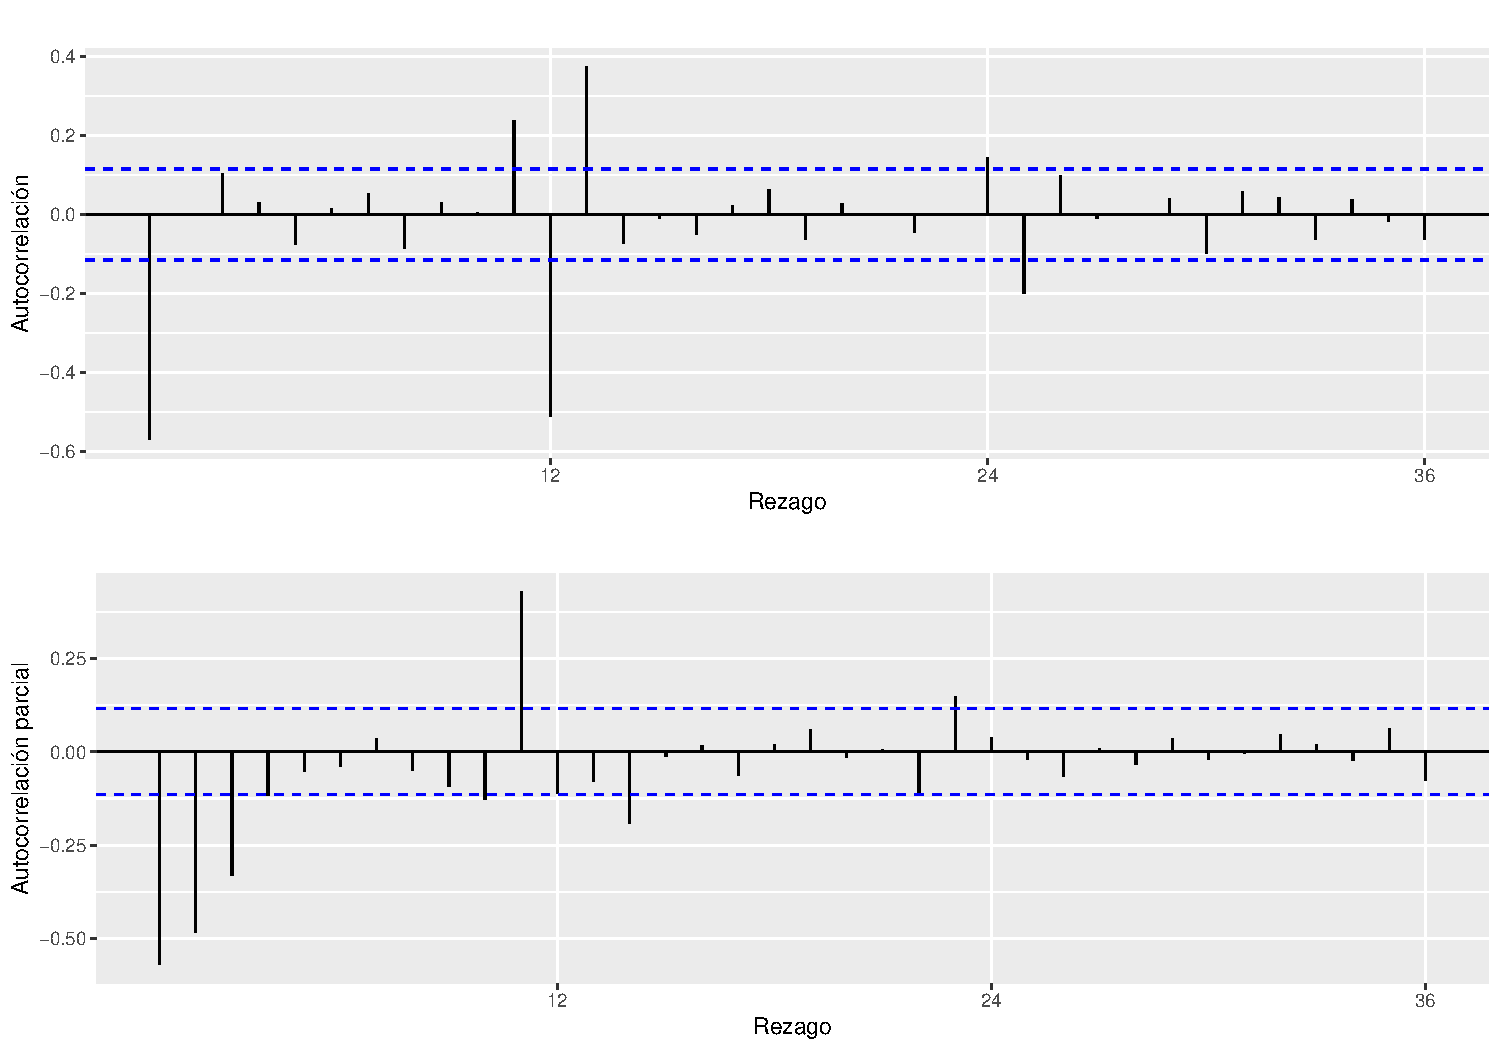
\includegraphics[width=0.7\linewidth]{presentacion_files/figure-beamer/unnamed-chunk-5-1} 

}

\caption{\label{dd_fac_facp} Funciones de Autocorrelación y Autocorrelación Parcial estimadas para la primera diferencia regular de la primera diferencia estacional del logaritmo del Gasto Público.}\label{fig:unnamed-chunk-5}
\end{figure}
\end{frame}

\begin{frame}{Identificación (2)}
\protect\hypertarget{identificaciuxf3n-2}{}
La convergencia de las funciones es mas consistente que en la serie con
diferencia estacional únicamente. A partir de estas funciones se
identifican 2 modelos adicionales, \textbf{SARIMA(0,1,2)(1,1,0)} y
\textbf{SARIMA(0,1,1)(0,1,1)}.

En este caso al haber ambas diferencias los parámetros \(d=1\) y \(D=1\)
son fijos. Con respecto a la parte regular, la FACP presenta los
primeros tres rezagos significativos, sin embargo se descarta un modelo
con parte AR de orden tan grande dado que la FAC no presenta un ruido
tan grande; de haber parte AR, la FAC no presentaria una convergencia
tan rápida como tiene a partir del rezago 2. En cambio, la convergencia
de la FACP es más lenta, lo cual sugiere un modelo con parte MA de orden
1 e incluso 2, por lo tanto \(q={1,2}\). Con respecto a la parte
estacional, las conclusiones son las mismas a la de la figura
\ref{fac_facp_estac}, la FAC y la FACP presenta el primer rezago
significativo dando lugar a dos posibilidades \(P=1\) o \(Q=1\).
\end{frame}

\begin{frame}{Variables regresoras}
\protect\hypertarget{variables-regresoras}{}
La etapa de identificación ha identificado 4 modelos posibles para
modelar la serie de Gasto Público. Estos modelos son en esta parte
estimados y comparados. Adicionalmente es incorporada al modelo una
variable regresora, los días de turismo, con el objetivo de capturar la
variabilidad de la serie generada en los marzos y abril de cada año, que
coincidie con el pago de los aguinaldos de los empleados públicos. La
figura \ref{gasto_2009-2013} representa la evolución del logaritmo del
Gasto Público entre enero 2009 y diciembre 2012, con las líneas
verticales punteadas marcando los meses de marzo y abril de cada año.
\end{frame}

\begin{frame}{Variable regresora: turismo}
\protect\hypertarget{variable-regresora-turismo}{}
\begin{figure}[H]

{\centering 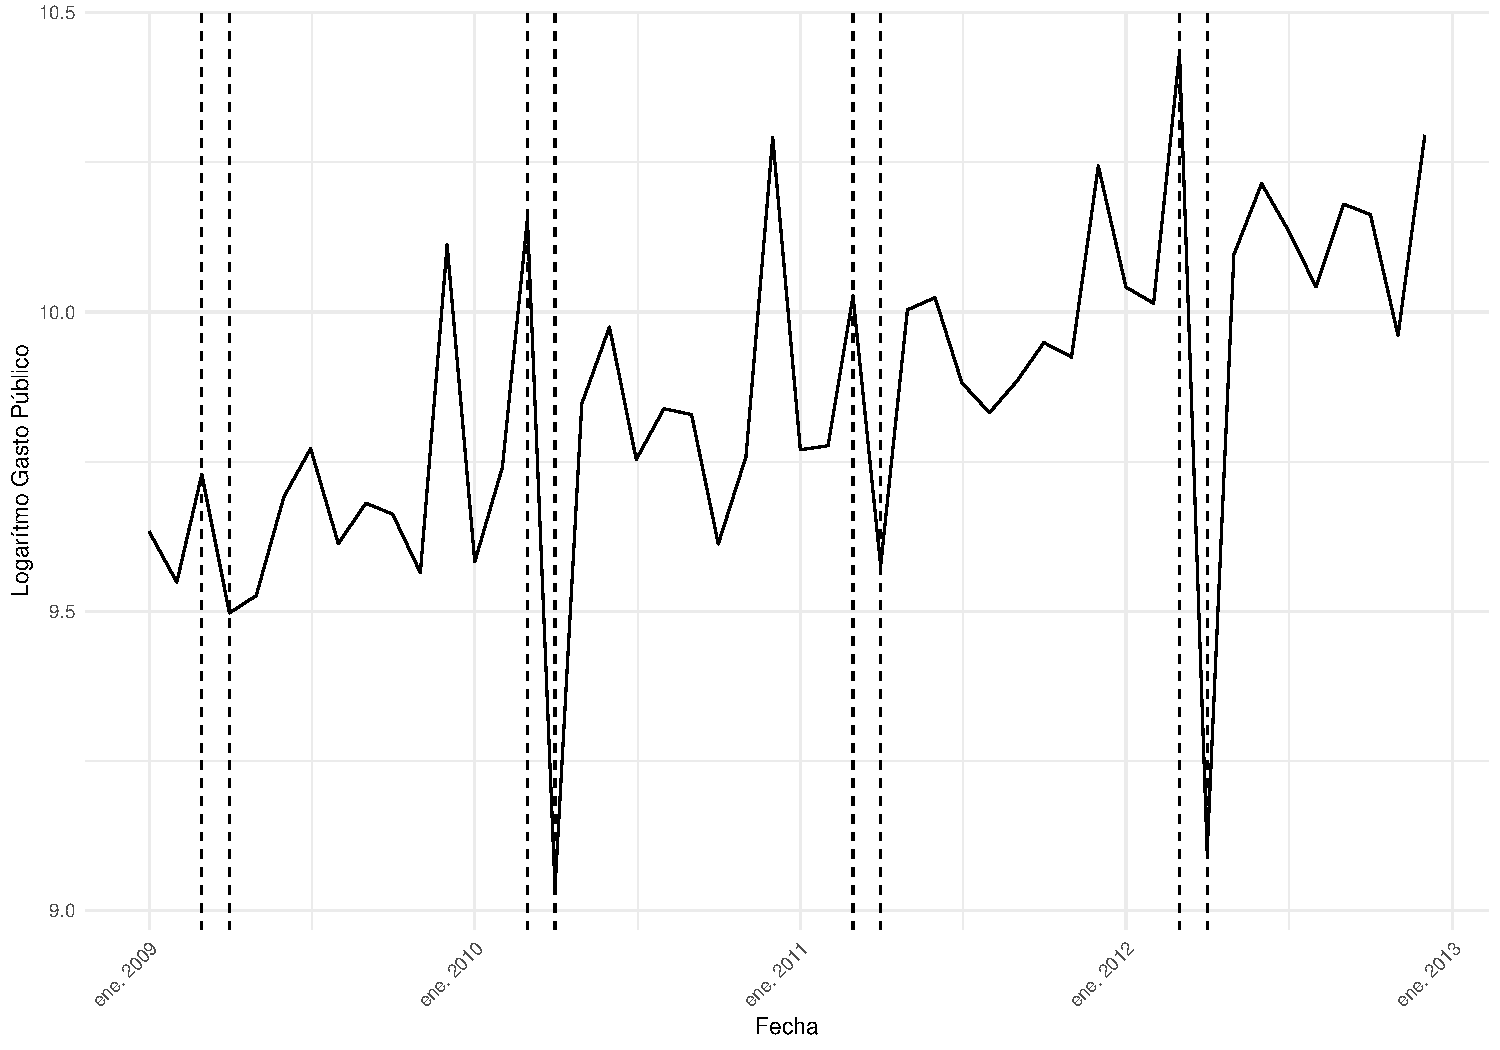
\includegraphics[width=0.85\linewidth]{presentacion_files/figure-beamer/gasto_2009-2012-1} 

}

\caption{\label{gasto_2009-2013} Evolución del Logarítmo del Gasto Público mensual entre enero 2009 y diciembre 2012.}\label{fig:gasto_2009-2012}
\end{figure}
\end{frame}

\begin{frame}{Variable regresora: turismo}
\protect\hypertarget{variable-regresora-turismo-1}{}
Dependiendo de cuando caen los días de turismo, determina el mes en el
que se efectuará el pago de los aguinaldos de los empleados públicos.
Esto puede generar un pago anticipado de los aguinaldos en determinado
mes, generando un alto gasto, y un gasto mucho menor al mes siguiente.
El cuadro \ref{tab:turismo} muestra los dias de turismo de cada año
entre 2009-2012:

\begin{table}[H]
\centering
\begin{tabular}{c c c c c}
\hline
 & 2009 & 2010 & 2011 & 2012 \\ \hline
Marzo & 0 & 3 & 0 & 0 \\ 
Abril & 7 & 4 & 7 & 7 \\ \hline
\end{tabular}
\caption{Días de tursimo en marzo y abril de 2009 a 2012.}
\label{tab:turismo}
\end{table}
\end{frame}

\begin{frame}{Estimación}
\protect\hypertarget{estimaciuxf3n}{}
El cuadro \ref{tab:models}, es un resúmen de la estimación de los 4
modelos SARIMA identificados, proporciona la varianza del modelo y la
significancia de sus componentes.

\begin{table}[H]
\centering
\resizebox{1\textwidth}{!}{
  \begin{tabular}{c c c c}
  \hline
  Modelo & SARIMA(p,d,q)(P,D,Q) + turismo & $\sigma^2$ & Significancia de los componentes \\ \hline
  1 & (0,0,1)(0,1,1) & 0.0493 & MA 1 no significativo \\ 
  2 & (0,0,1)(1,1,0) & 0.0484 & MA 1 no significativo \\ 
  3 & (0,1,2)(1,1,0) & 0.0240 & Todos significativos \\ 
  4 & (0,1,1)(0,1,1) & 0.0271 & Todos significativos \\ \hline
  \end{tabular}
}
\caption{Estimación de modelos SARIMA.}
\label{tab:models}
\end{table}

Los dos modelos que incluyen únicamente la diferencia estacional,
aparentan ser peores que los modelos con diferencias regular y
estacional en términos de varianza del modelo, a su vez el componente MA
de orden 1 en la parte regular de los dos primeros modelos, suele ser
rechazada al 5\% de nivel de significación.
\end{frame}

\begin{frame}{Diagnóstico}
\protect\hypertarget{diagnuxf3stico}{}
En esta etapa, los 4 modelos estimados son diagnosticados para verificar
si cumplen con los supuestos de ruido blanco es decir incorrelación y
normalidad de los resiudos.

El análisis de las funciones de autocorrelación y autocorrelación
parcial de los residuos permite observar la autocorrelación de los
mismos, y acompañado del test de Ljung-Box, se verifica la
incorrelación.

Por otro lado los tests de Shapiro-Wilks y Jarque-Bera, permiten
verificar la normalidad de los residuos.
\end{frame}

\begin{frame}{Diagnóstico: Residuos y residuos estandarizados}
\protect\hypertarget{diagnuxf3stico-residuos-y-residuos-estandarizados}{}
\begin{figure}[H]

{\centering 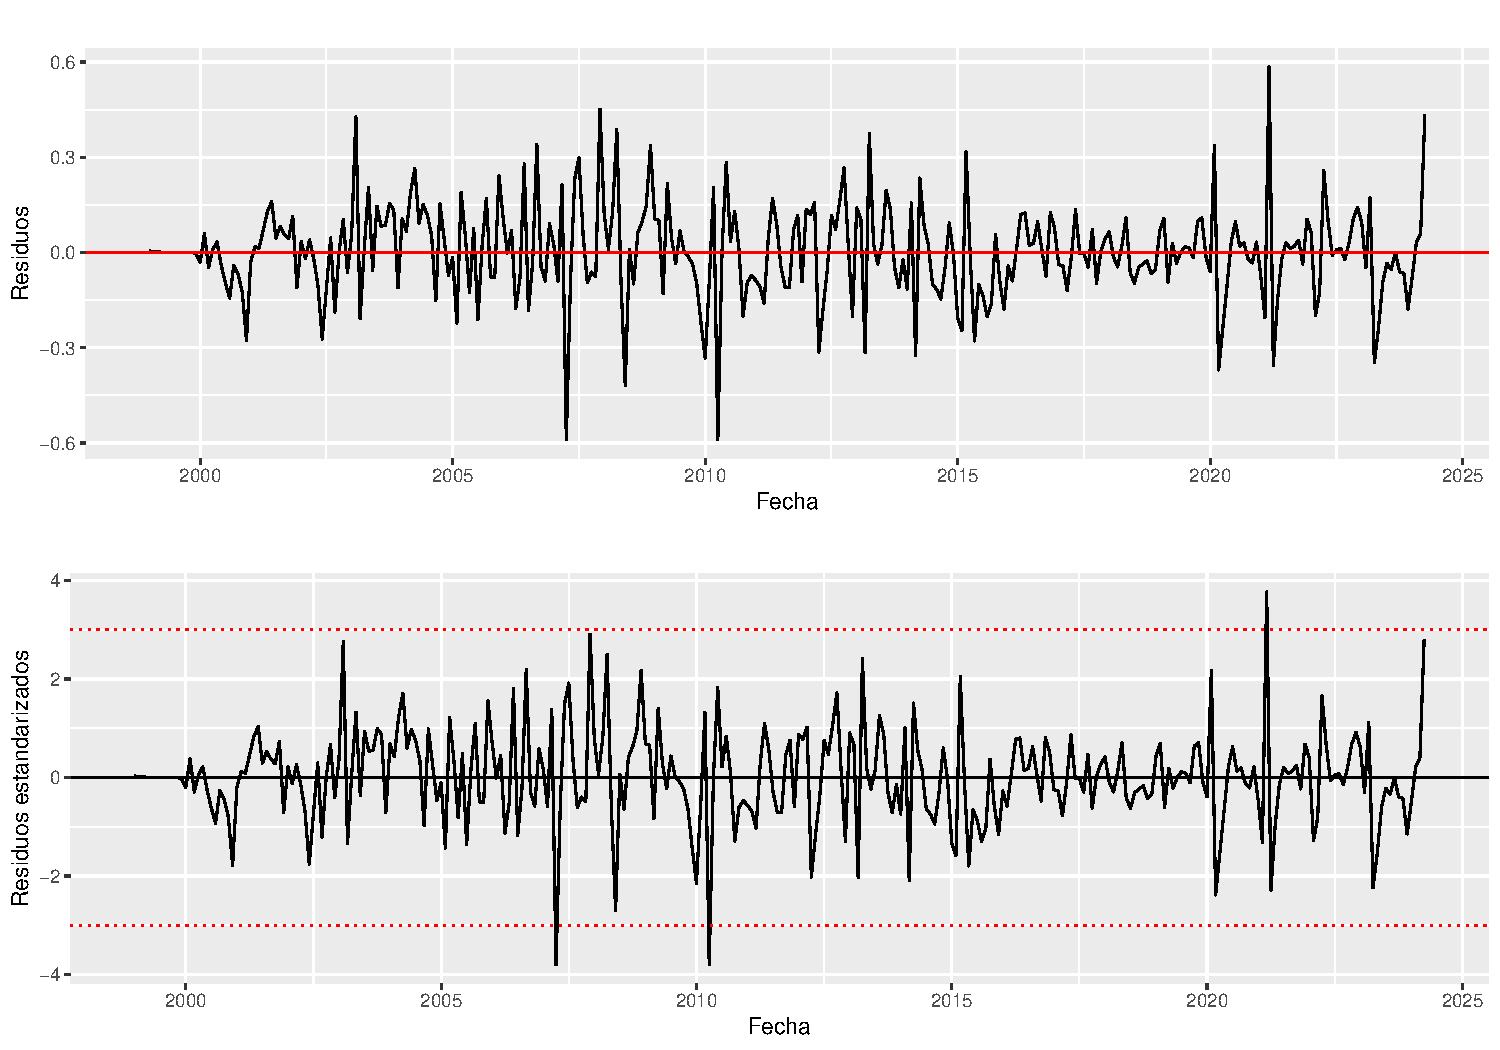
\includegraphics[width=0.75\linewidth]{presentacion_files/figure-beamer/unnamed-chunk-6-1} 

}

\caption{\label{residuos3} Residuos normales y estandarizados de un modelo SARIMA(0,1,2)(1,1,0) para el logaritmo del Gasto Público.}\label{fig:unnamed-chunk-6}
\end{figure}
\end{frame}

\begin{frame}{Diagnóstico:Función de autocorrelación y autocorrelación
parcial de los residuos}
\protect\hypertarget{diagnuxf3sticofunciuxf3n-de-autocorrelaciuxf3n-y-autocorrelaciuxf3n-parcial-de-los-residuos}{}
\begin{figure}[H]

{\centering 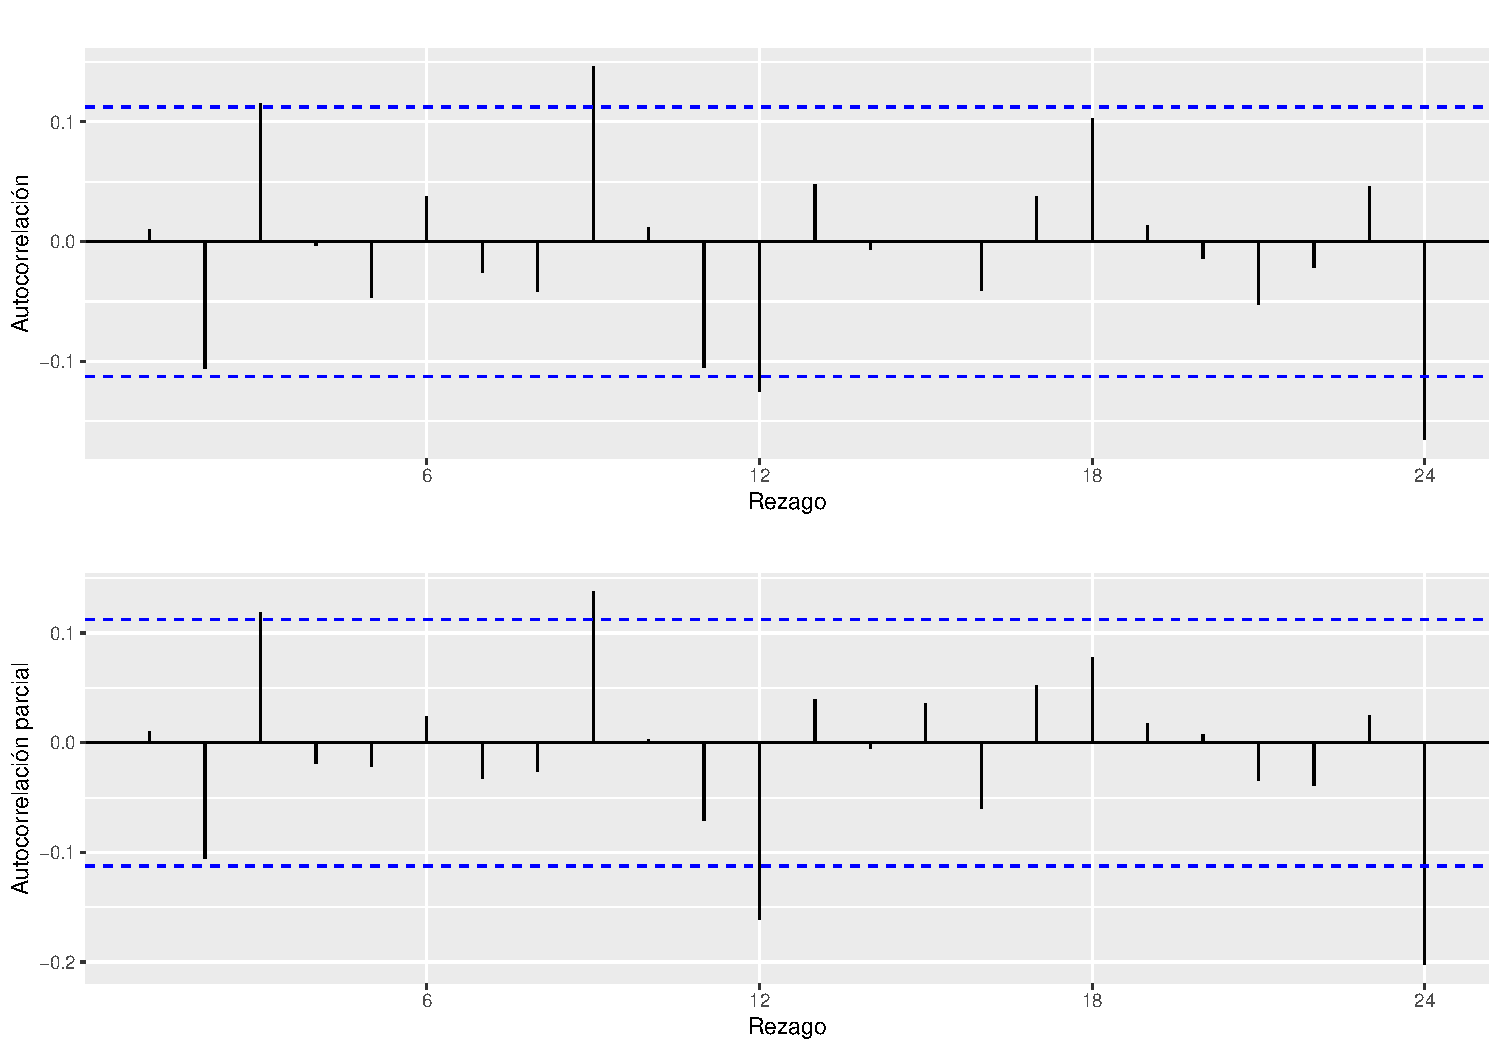
\includegraphics[width=0.75\linewidth]{presentacion_files/figure-beamer/unnamed-chunk-8-1} 

}

\caption{\label{facyp_r3} Funciones de Autocorrelación y Autocorrelación Parcial estimadas de los residuos de un modelo SARIMA(0,1,2)(1,1,0) para el logaritmo del Gasto Público.}\label{fig:unnamed-chunk-8}
\end{figure}
\end{frame}

\begin{frame}{Diagnóstico: Tests de Ljung-Box y Shapiro-Wilks}
\protect\hypertarget{diagnuxf3stico-tests-de-ljung-box-y-shapiro-wilks}{}
Veánse los resultados de la incorrelación y normalidad de los residuos
en el cuadro \ref{tab:diagnostico}.

\begin{table}[H]
\centering
\resizebox{1\textwidth}{!}{
  \begin{tabular}{c c c c}
  \hline
  Modelo & SARIMA(p,d,q)(P,D,Q) + turismo & Incorrelación & Normalidad \\ \hline
  1 & (0,0,1)(0,1,1) & No & No \\ 
  2 & (0,0,1)(1,1,0) & No & No \\ 
  3 & (0,1,2)(1,1,0) & No & No \\ 
  4 & (0,1,1)(0,1,1) & No & No \\ \hline
  \end{tabular}
}
\caption{Diagnostico de modelos SARIMA.}
\label{tab:diagnostico}
\end{table}
\end{frame}

\begin{frame}{Diagnóstico: Detección de outliers}
\protect\hypertarget{diagnuxf3stico-detecciuxf3n-de-outliers}{}
Los outliers detectados para cada modelo son las siguientes
observaciones:

\begin{itemize}
\tightlist
\item
  Modelo 1

  \begin{itemize}
  \tightlist
  \item
    AO: 51, 100, 136, 160, 195, 255, 267, 280, 304.
  \item
    LS: 117, 159.
  \item
    TC: 254
  \end{itemize}
\item
  Modelo 2

  \begin{itemize}
  \tightlist
  \item
    AO: 51, 100, 136, 160, 195, 255, 267, 280, 304.
  \item
    TC: 159, 254, 291.
  \end{itemize}
\item
  Modelo 3

  \begin{itemize}
  \tightlist
  \item
    AO: 100, 160, 292.
  \end{itemize}
\item
  Modelo 4

  \begin{itemize}
  \tightlist
  \item
    AO: 51, 100, 136, 160, 195, 255, 268, 279, 292.
  \end{itemize}
\end{itemize}
\end{frame}

\begin{frame}{Reestimación}
\protect\hypertarget{reestimaciuxf3n}{}
\begin{table}[H]
\centering
\resizebox{1\textwidth}{!}{
  \begin{tabular}{c c c c}
  \hline
  Modelo & SARIMA(p,d,q)(P,D,Q) + turismo + outliers & $\sigma^2$ & Significancia de los componentes \\ \hline
  1 & (0,0,1)(0,1,1) & 0.0227 & s\_MA 1 no significativo \\ 
  2 & (0,0,1)(1,1,0) & 0.0226 & Todos significativos \\ 
  3 & (0,1,2)(1,1,0) & 0.0205 & Regresor turismo no significativo \\ 
  4 & (0,1,1)(0,1,1) & 0.0156 & Todos significativos \\ \hline
  \end{tabular}
}
\caption{Reestimación de modelos SARIMA con intervención de outliers.}
\label{tab:models2}
\end{table}
\end{frame}

\begin{frame}{Reestimación (2)}
\protect\hypertarget{reestimaciuxf3n-2}{}
\begin{table}[H]
\centering
\resizebox{1\textwidth}{!}{
  \begin{tabular}{c c c c}
  \hline
  Modelo & SARIMA(p,d,q)(P,D,Q) + outliers & $\sigma^2$ & Significancia de los componentes \\ \hline
  1 & (0,0,1)(0,1,0) + turismo & 0.0226 & Todos significativos \\ 
  3 & (0,1,2)(1,1,0) & 0.0205 & Todos significativos \\ \hline
  \end{tabular}
}
\caption{Reestimación de modelos SARIMA con intervención de outliers.}
\label{tab:models3}
\end{table}
\end{frame}

\begin{frame}{Diagnóstico: Residuos y residuos estandarizados}
\protect\hypertarget{diagnuxf3stico-residuos-y-residuos-estandarizados-1}{}
\begin{figure}[H]

{\centering 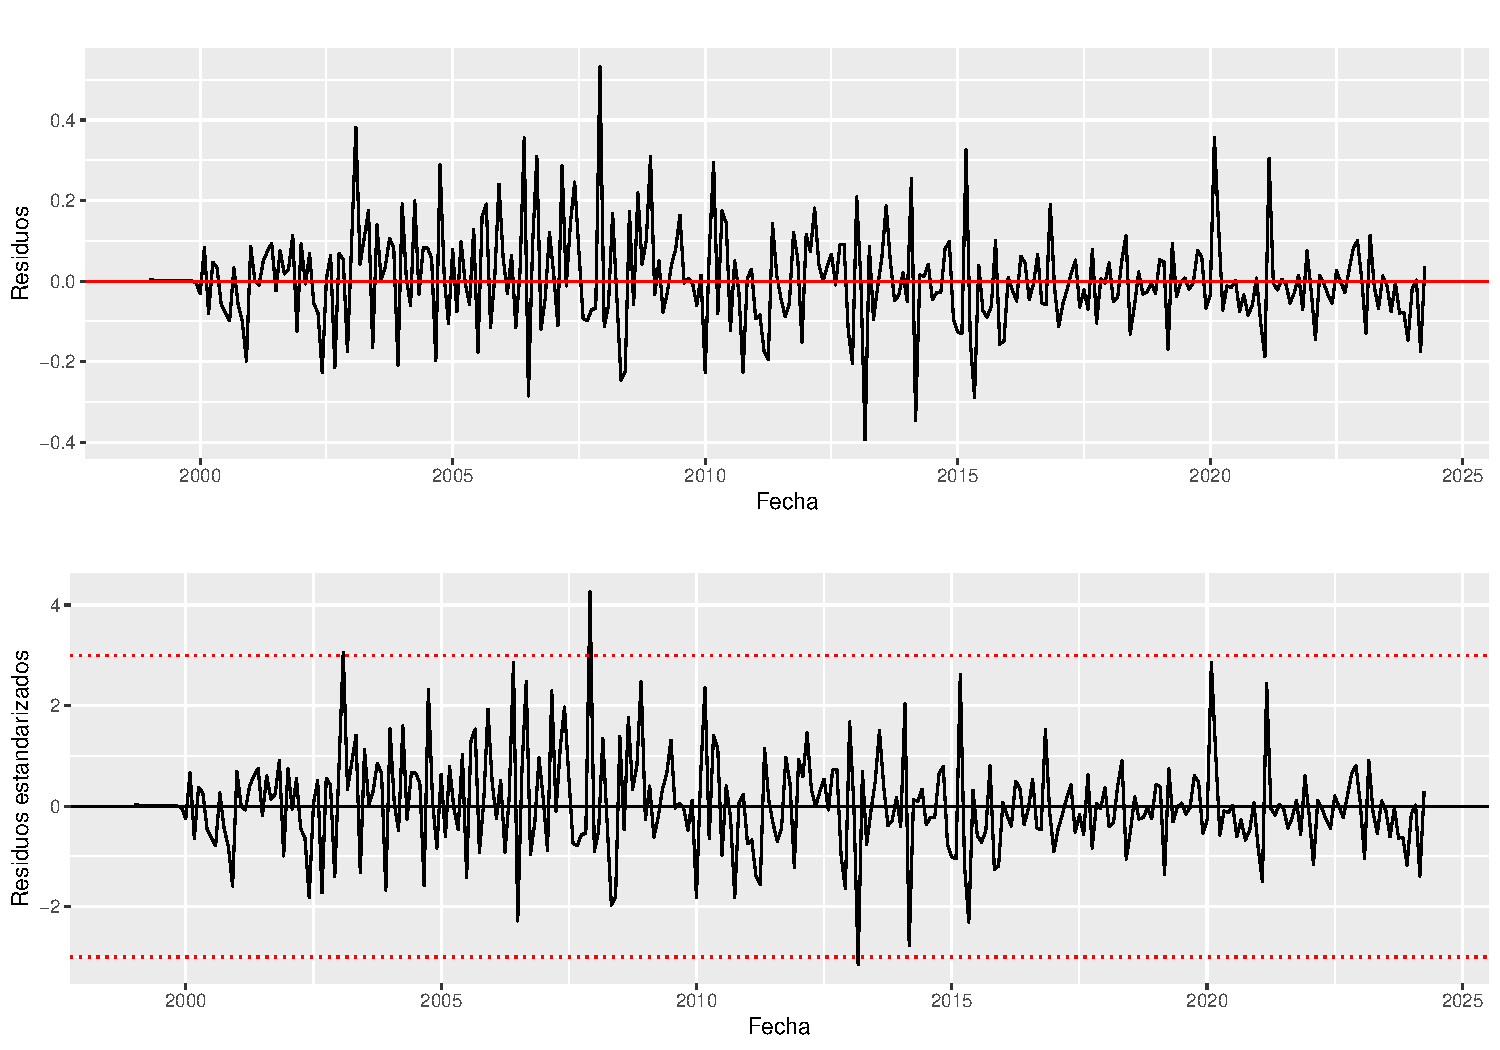
\includegraphics[width=0.85\linewidth]{presentacion_files/figure-beamer/unnamed-chunk-15-1} 

}

\caption{\label{residuos4} Residuos normales y estandarizados de un modelo SARIMA(0,1,1)(0,1,1) intervenido para el logaritmo del Gasto Público.}\label{fig:unnamed-chunk-15}
\end{figure}
\end{frame}

\begin{frame}{Diagnostico: Función de autocorrelación y autocorrelación
parcial de los residuos}
\protect\hypertarget{diagnostico-funciuxf3n-de-autocorrelaciuxf3n-y-autocorrelaciuxf3n-parcial-de-los-residuos}{}
\begin{figure}[H]

{\centering 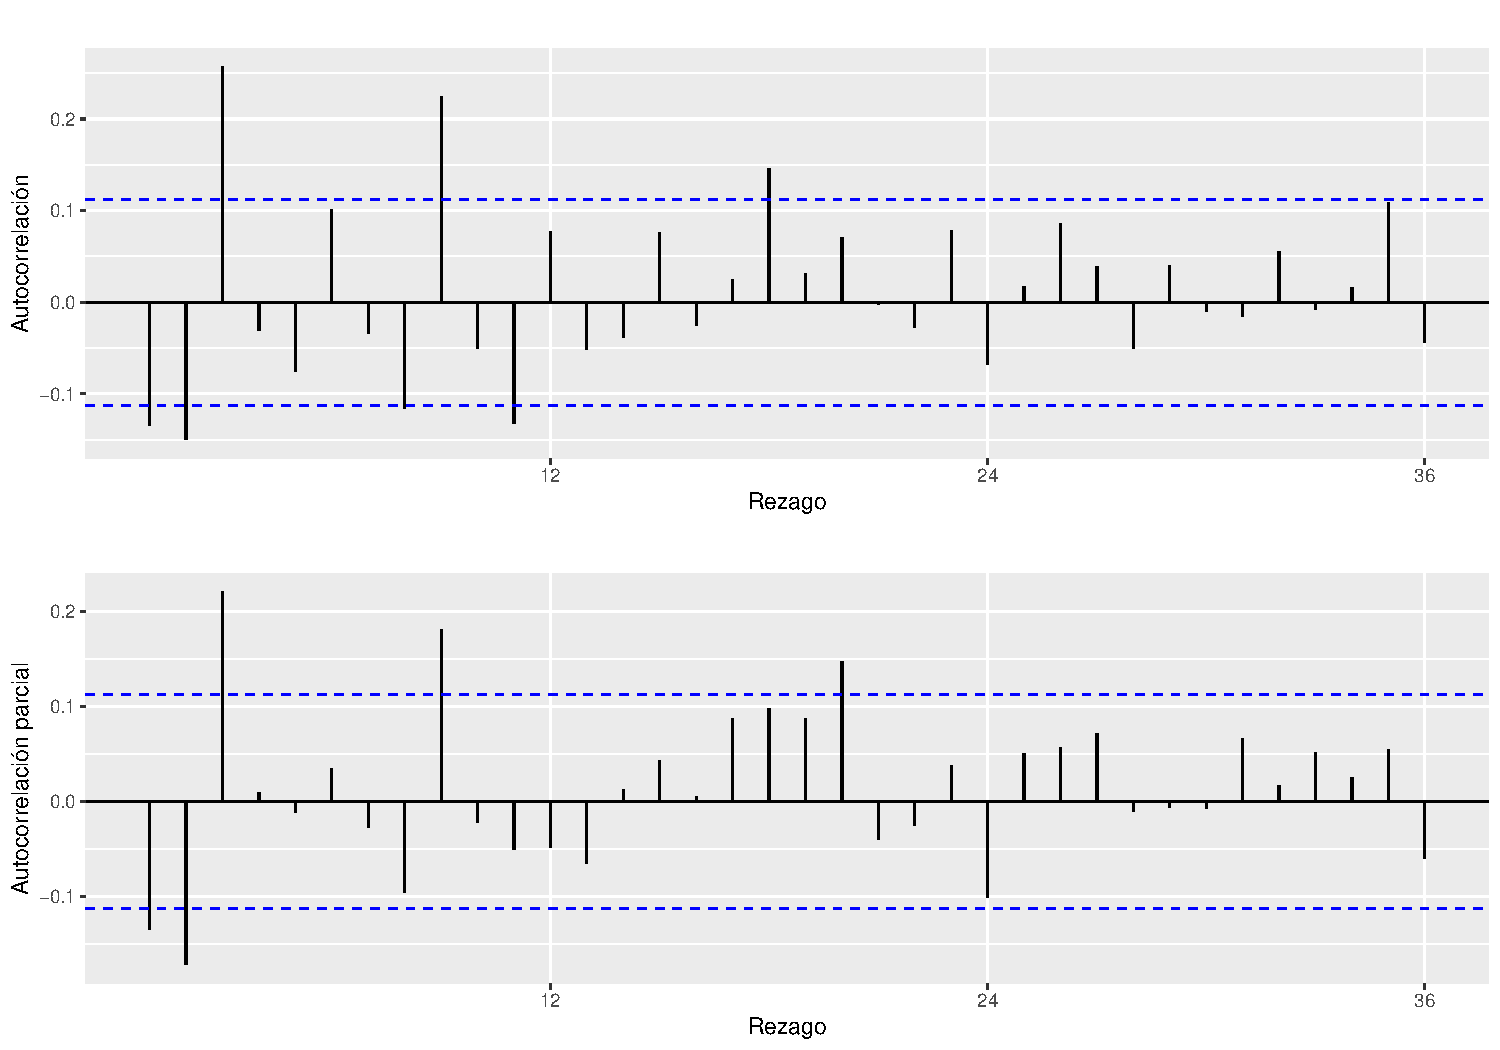
\includegraphics[width=0.75\linewidth]{presentacion_files/figure-beamer/unnamed-chunk-16-1} 

}

\caption{\label{facyp_r4} Funciones de Autocorrelación y Autocorrelación Parcial estimadas de los residuos de un modelo SARIMA(0,1,1)(0,1,1) intervenido para el logaritmo del Gasto Público.}\label{fig:unnamed-chunk-16}
\end{figure}
\end{frame}

\begin{frame}{Diagnostico: Tests de Ljung-Box y Shapiro-Wilks}
\protect\hypertarget{diagnostico-tests-de-ljung-box-y-shapiro-wilks}{}
\begin{table}[H]
\centering
\resizebox{1\textwidth}{!}{
\begin{tabular}{c c c c}
\hline
Modelo & SARIMA(p,d,q)(P,D,Q) + outliers & Incorrelación & Normalidad \\ \hline
1 & (0,0,1)(0,1,0) + tursimo & No & No \\ 
2 & (0,0,1)(1,1,0) + turismo & No & No \\ 
3 & (0,1,2)(1,1,0) & No & No \\ 
4 & (0,1,1)(0,1,1) + turismo & No & No \\ \hline
\end{tabular}
}
\caption{Diagnosticos de modelos SARIMA.}
\label{tab:diagnostico2}
\end{table}
\end{frame}

\begin{frame}{Diagnóstico: Histograma de los residuos}
\protect\hypertarget{diagnuxf3stico-histograma-de-los-residuos}{}
\begin{figure}[H]

{\centering 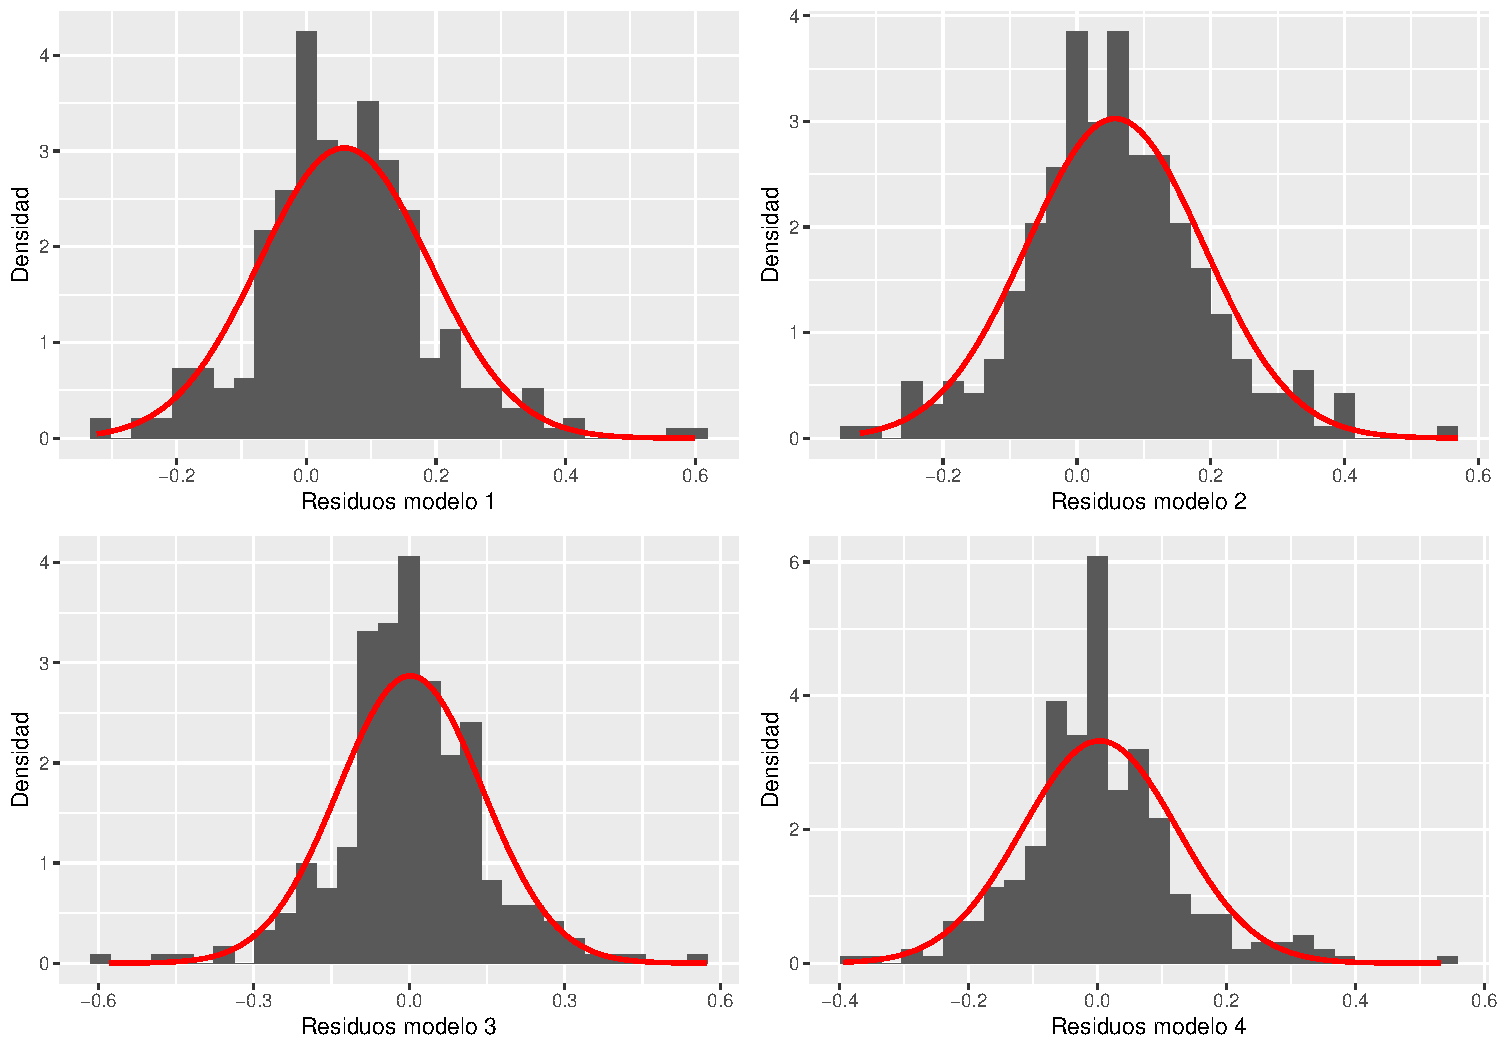
\includegraphics[width=0.8\linewidth]{presentacion_files/figure-beamer/unnamed-chunk-19-1} 

}

\caption{\label{norms} Histograma de los residuos de los modelos reestimados SARIMA intervenido spara el logaritmo del Gasto Público. La línea roja corresponde a una densidad normal con media y desvío muestrales igual al de los residuos.}\label{fig:unnamed-chunk-19}
\end{figure}
\end{frame}

\begin{frame}{Predicción}
\protect\hypertarget{predicciuxf3n}{}
Puntos a tener en cuenta:

\begin{itemize}
\item
  Función de pérdida: simétrica.
\item
  Horizonte de predicción: 12 meses.
\item
  Conjunto de entrenamiento: hasta abril de 2023.
\item
  Conjunto de testeo: desde mayo de 2023.
\item
  Variables exógenas: turismo y outliers.
\end{itemize}
\end{frame}

\begin{frame}{Predicción (2)}
\protect\hypertarget{predicciuxf3n-2}{}
Las métricas de error que se utilizarán para comparar los modelos son:

\begin{itemize}
\item
  Error absoluto medio (MAE): mide la magnitud absoluta promedio del
  desvío de la predicción del valor real.
\item
  Error porcentual absoluto medio (MAPE): mide la magnitud promedio del
  desvío de la predicción del valor real en términos porcentuales.
\item
  Error medio absoluto escalado (MASE): mide la magnitud promedio del
  desvío de la predicción del valor real, escalada por el MAE del
  conjunto de entrenamiento.
\end{itemize}

Un valor más cercano a cero indica una mejor predicción para las tres
métricas.
\end{frame}

\begin{frame}{Predicción de los modelos 1 y 2}
\protect\hypertarget{predicciuxf3n-de-los-modelos-1-y-2}{}
\textbackslash begin\{figure\}{[}H{]}

\{\centering 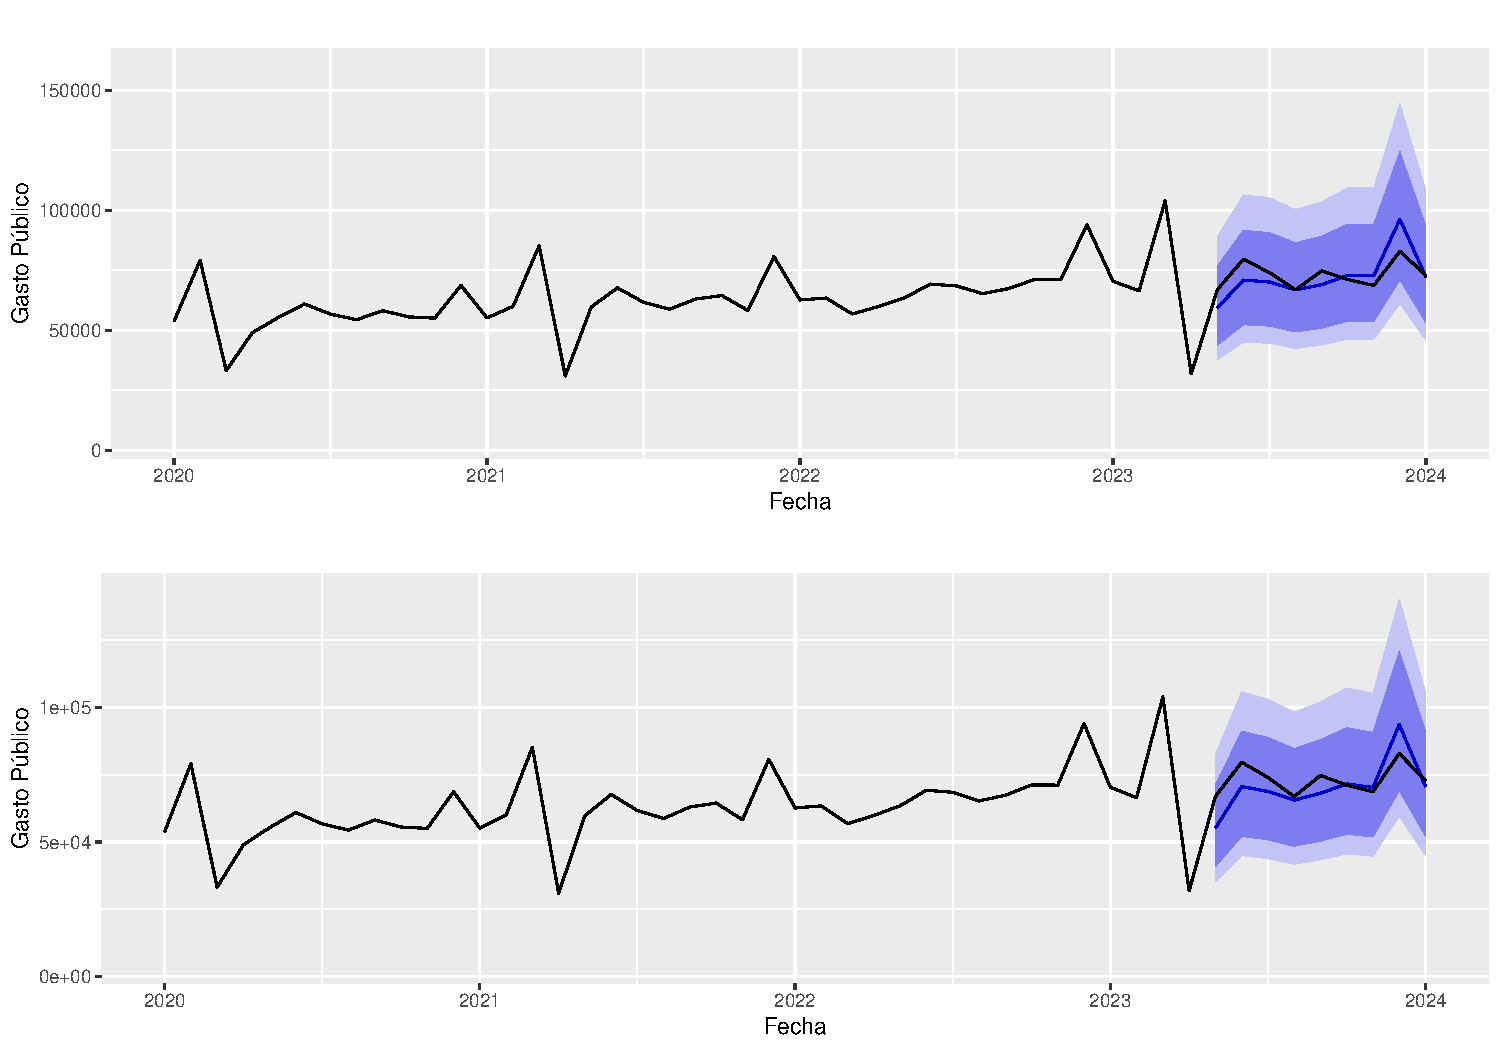
\includegraphics[width=0.95\linewidth]{presentacion_files/figure-beamer/unnamed-chunk-23-1}

\}

\textbackslash caption\{\label{pred12} Predicciones en el conjunto de
prueba del Gasto Público, para los modelos 1 y 2 respectivamente. La
línea azul corresponde a las predicciones y la negra a los datos reales.
El azul mas claro correspode al intervalo de predicción al 95\% de
confianza y la mas oscura al 80.\}\label{fig:unnamed-chunk-23}
\textbackslash end\{figure\}
\end{frame}

\begin{frame}{Predicción de los modelos 3 y 4}
\protect\hypertarget{predicciuxf3n-de-los-modelos-3-y-4}{}
\textbackslash begin\{figure\}{[}H{]}

\{\centering 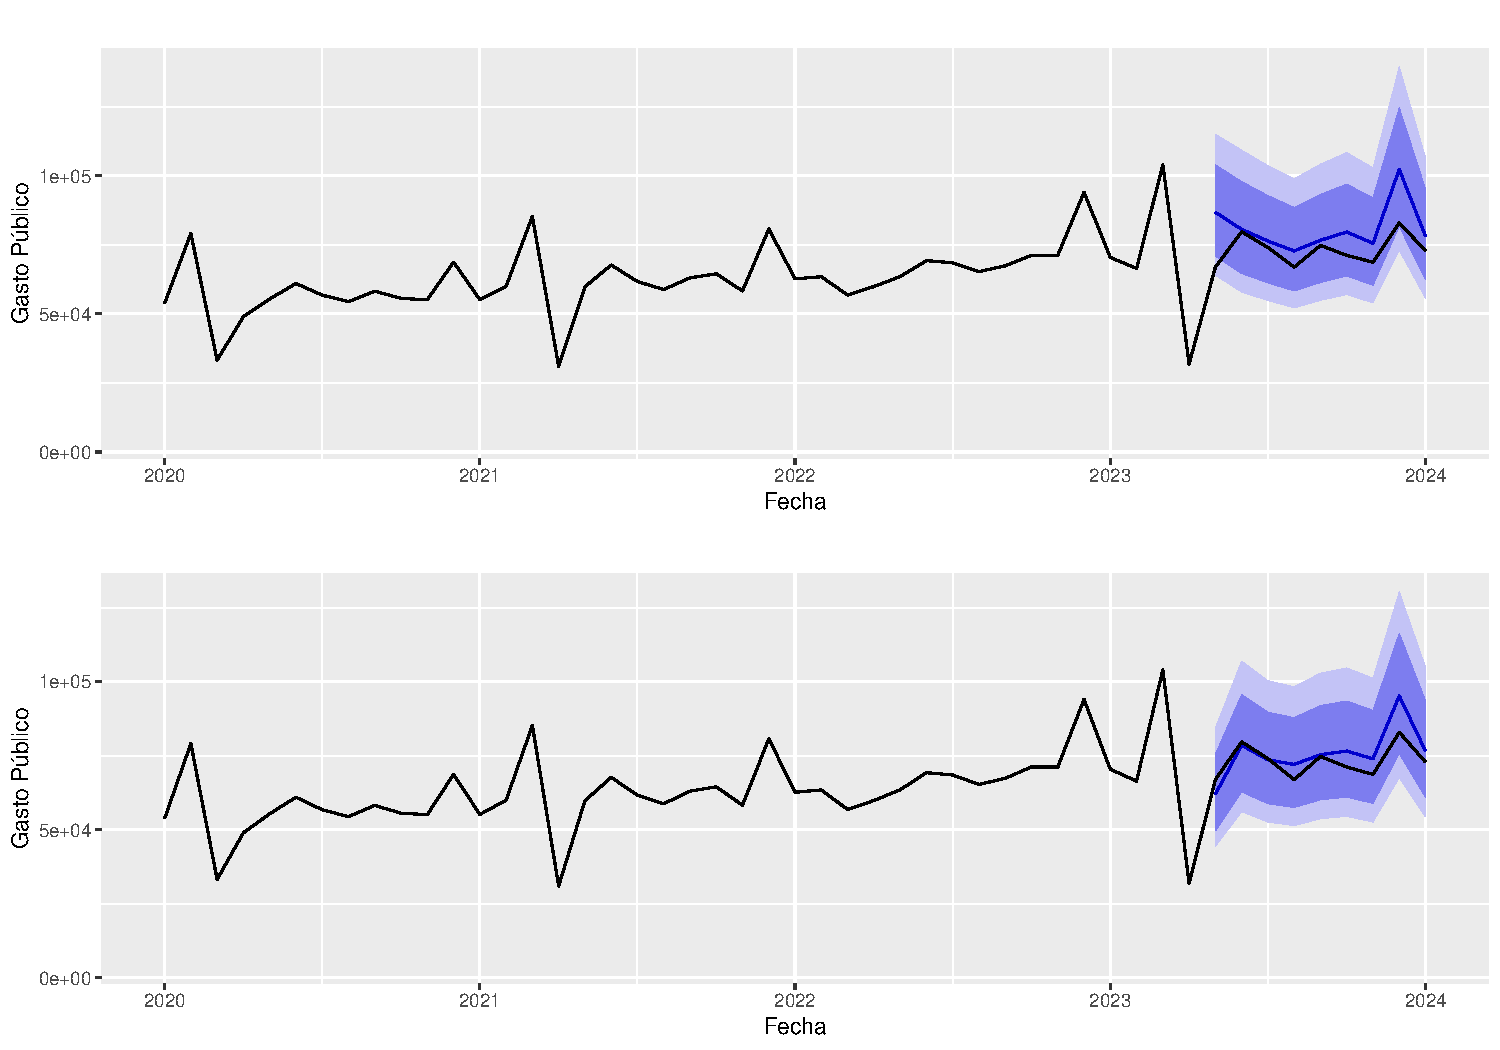
\includegraphics[width=0.95\linewidth]{presentacion_files/figure-beamer/unnamed-chunk-24-1}

\}

\textbackslash caption\{\label{pred34} Predicciones en el conjunto de
prueba del Gasto Público, para los modelos 3 y 4 respectivamente. La
línea azul corresponde a las predicciones y la negra a los datos reales.
El azul mas claro correspode al intervalo de predicción al 95\% de
confianza y la mas oscura al 80.\}\label{fig:unnamed-chunk-24}
\textbackslash end\{figure\}
\end{frame}

\begin{frame}{Predicción: Métricas de error}
\protect\hypertarget{predicciuxf3n-muxe9tricas-de-error}{}
\begin{table}[H]
\centering
\resizebox{1\textwidth}{!}{
  \begin{tabular}{c c c c c c}
  \hline
  Modelo & Conjunto & MAE & MAPE & MASE \\ \hline
  1 & Training  & 3541 & 12.85 & 0.868 \\ 
  1 & Test      & 10870 & 13.98 & 2.664 \\ \hline
  2 & Training  & 3565 & 13.10 & 0.874 \\ 
  2 & Test      & 9909 & 12.84 & 2.429 \\ \hline
  3 & Training  & 2757 & 10.92 & 0.676 \\ 
  3 & Test      & 9333 & 12.45 & 2.288 \\ \hline
  4 & Training  & 2729 & 10.87 & 0.669 \\ 
  4 & Test      & 6829 & 8.93 & 1.674 \\ \hline
  \end{tabular}
}
\caption{Resultados de error de predicción para los diferentes modelos.}
\label{tab:metricas}
\end{table}
\end{frame}

\begin{frame}{Conclusiones}
\protect\hypertarget{conclusiones}{}
En base a los resultados obtenidos, se puede concluir que el modelo 4
(entre los presentados) es el que presenta un mejor desempeño en los
datos. Este modelo es un SARIMA(0,1,1)(0,1,1) con un regresor turismo y
la inclusión de outliers detectados.

Se ha logrado llegar a resultados positivos, mas alla de la falta de
cumplimiento de los supuestos de los residuos respecto a la
incorrelación y normalidad de los residuos. Los puntos atípicos
presentes en la serie, han sido correctamente identificados y tratados
en los modelos, lo cual ha permitido mejorar la calidad de las
estimaciones.
\end{frame}

\begin{frame}{Comentarios Finales}
\protect\hypertarget{comentarios}{}
Hubiese estado bueno que al identificar los outliers aparte de haber
mejorado la estimación, hubiese ayudado al cumplimiento de la
incorrelación y normalidad de los residuos.

La predicción realizada en el conjunto de testeo, respondió
correctamente, presentando un error de predicción dentro de las
expectativas. El modelo 3 presenta una predicción rara de la primer
observación que solo queda contenida en el intervalo de predicción al
95\% de confianza, se desconoce el motivo de este comportamiento.

A efectos futuros, se sugiere probar las siguientes combinaciones de
modelos que quedaron pendientes de estimar y diagnosticar,
SARIMA(p,d,q)(P,D,Q):

\begin{itemize}
\item
  (0,1,2) (0,1,1)
\item
  (0,1,1) (1,1,0)
\end{itemize}
\end{frame}

\begin{frame}{Bibliografía}
\protect\hypertarget{bibliografuxeda}{}
\hypertarget{refs}{}
\begin{CSLReferences}{1}{0}
\leavevmode\vadjust pre{\hypertarget{ref-box1994time}{}}%
Box, G. E. P., G. M. Jenkins, y G. C. Reinsel. 1994. \emph{Time Series
Analysis; Forecasting and Control}. 3rd ed. Englewood Cliff, New Jersey:
Prentice Hall.

\leavevmode\vadjust pre{\hypertarget{ref-MEFUruguay}{}}%
Ministerio de Economía y Finanzas. 2024. {«{Información y Resultados del
Sector Público}»}.
\url{https://www.gub.uy/ministerio-economia-finanzas/datos-y-estadisticas/estadisticas/informacion-resultados-del-sector-publico}.

\end{CSLReferences}
\end{frame}

\begin{frame}{}
\protect\hypertarget{section}{}
\centering

¡Muchas Gracias!
\end{frame}

\end{document}
